\section{\textit{Cross-Checks} for QCD estimation in 2J1T} 
\label{app:qcdcrosschecks}
\subsection{Effect of nonQCD MC subtraction}
{
\begin{figure}[h!]
\resizebox{ \textwidth}{!}{
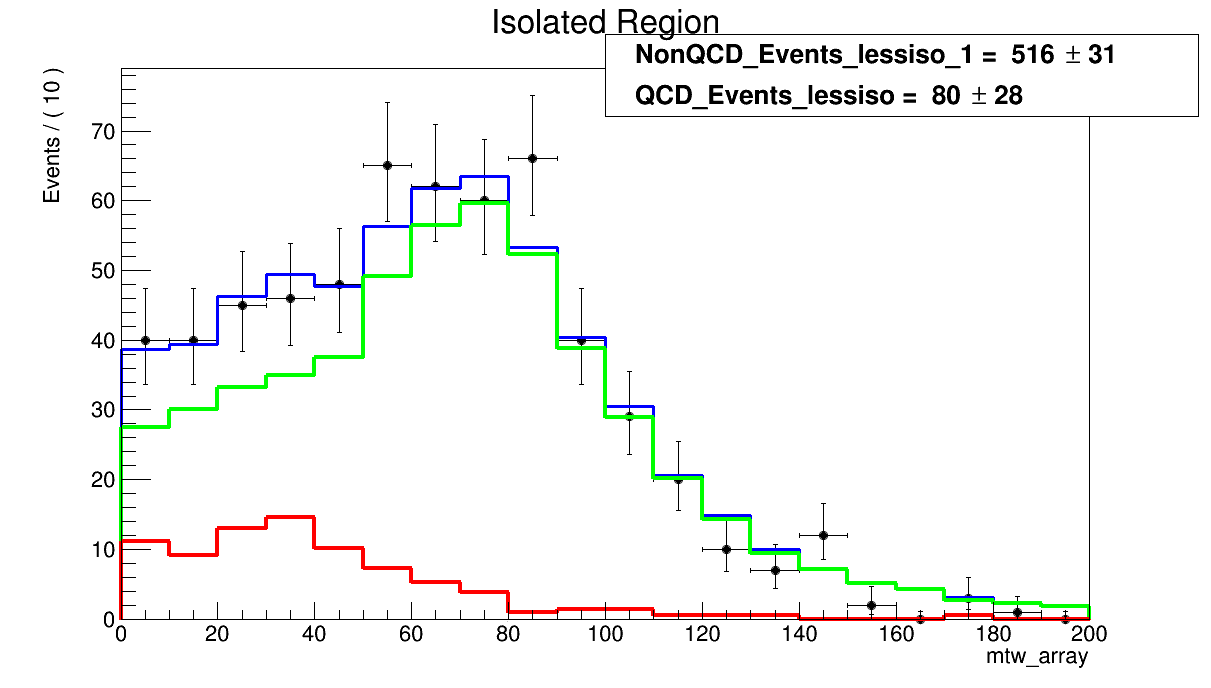
\includegraphics[scale=0.2]{figures/2J1T/MTW_fit_2j1t_lessiso_inclusive_mTop_range_NononQCDsubtraction}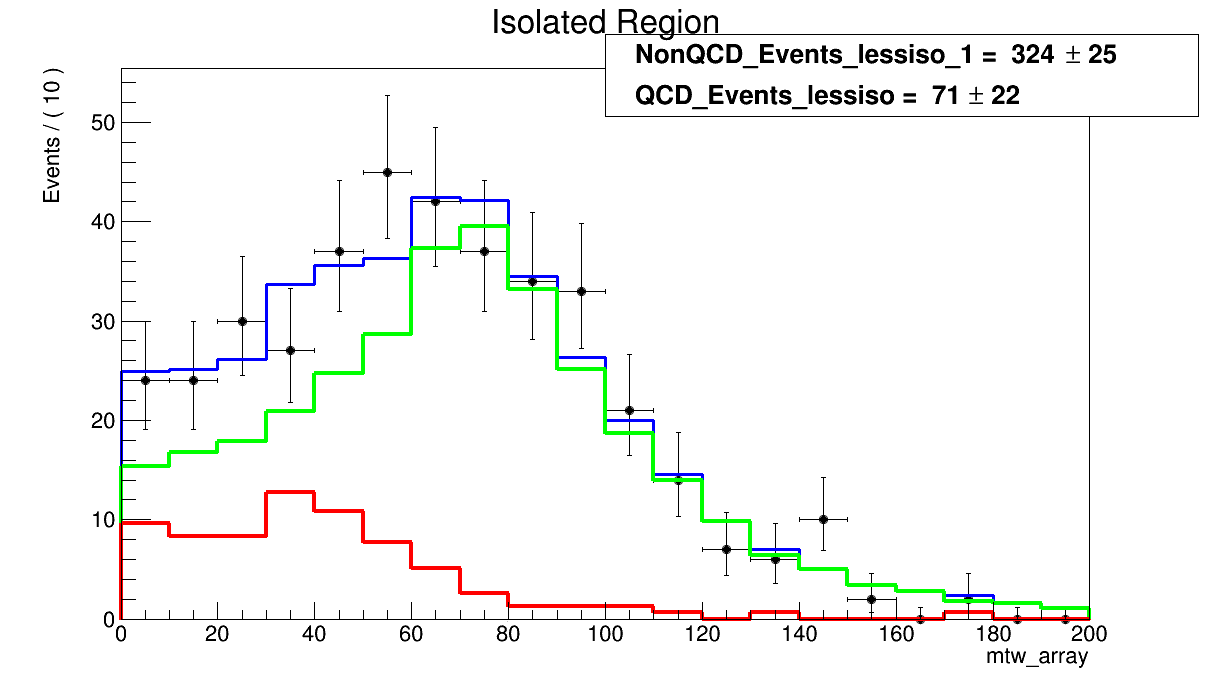
\includegraphics[scale=0.2]{figures/2J1T/MTW_fit_2j1t_lessiso_SR_NononQCDsubtraction}

\begin{centering}
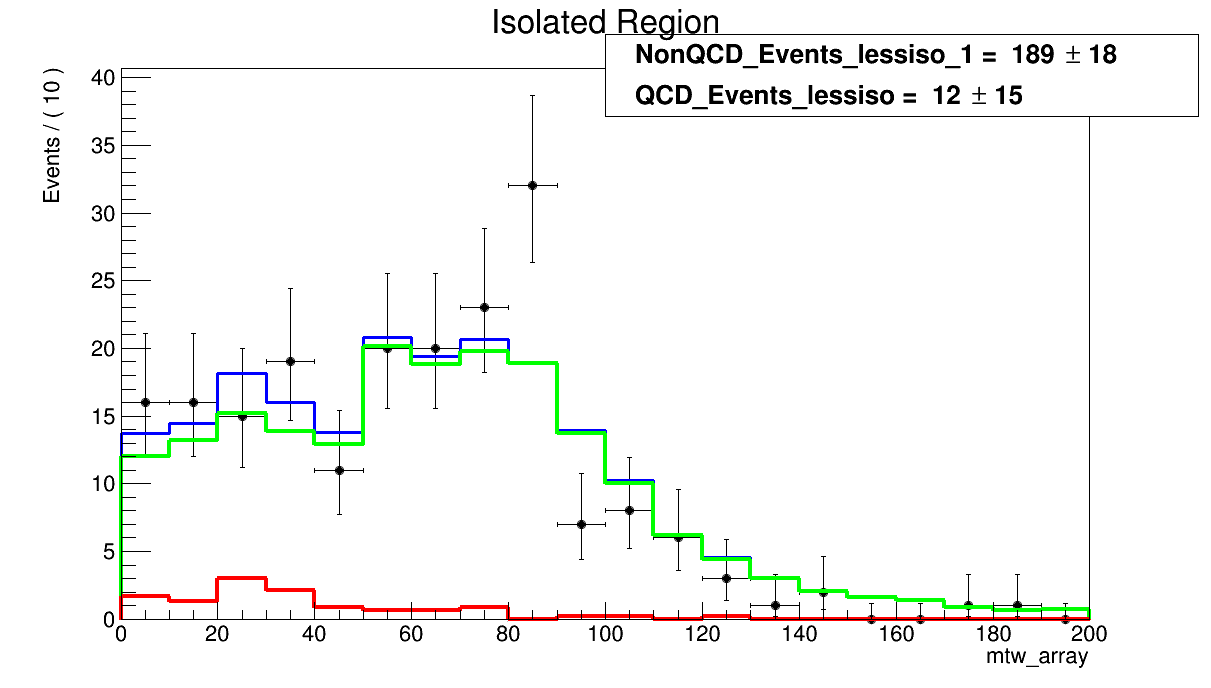
\includegraphics[scale=0.2]{figures/2J1T/MTW_fit_2j1t_lessiso_SB_NononQCDsubtraction}
\par\end{centering}
}
\resizebox{ \textwidth}{!}{
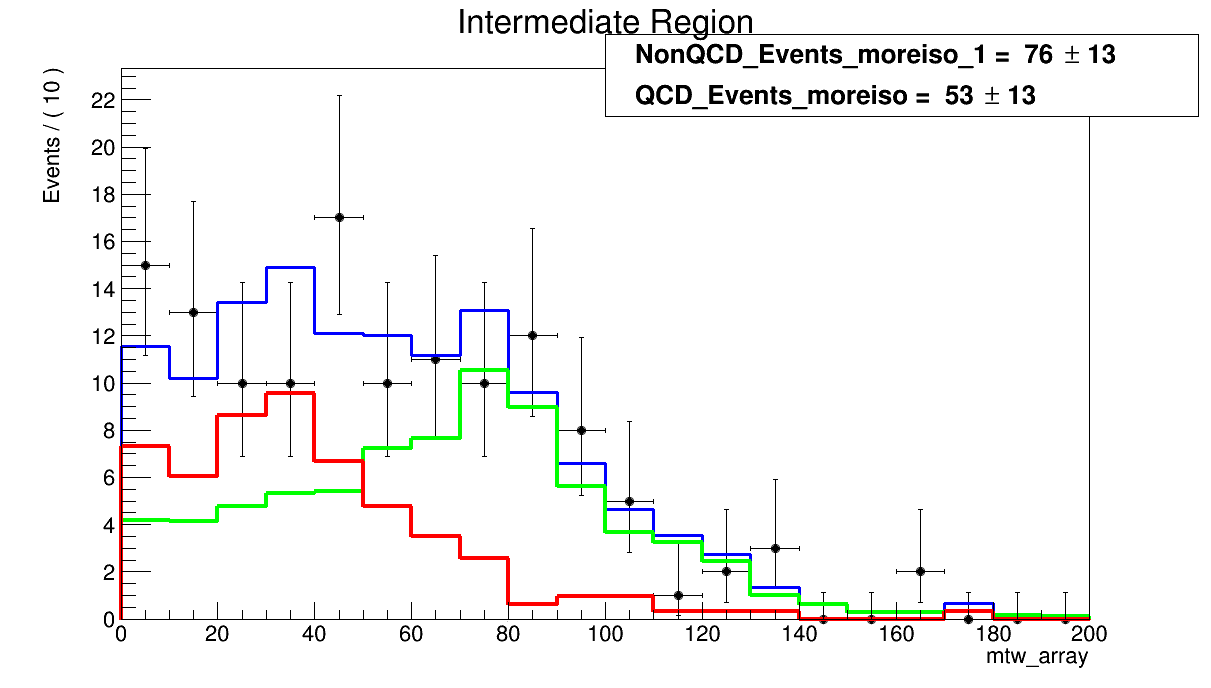
\includegraphics[scale=0.2]{figures/2J1T/MTW_fit_2j1t_moreiso_inclusive_mTop_range_NononQCDsubtraction}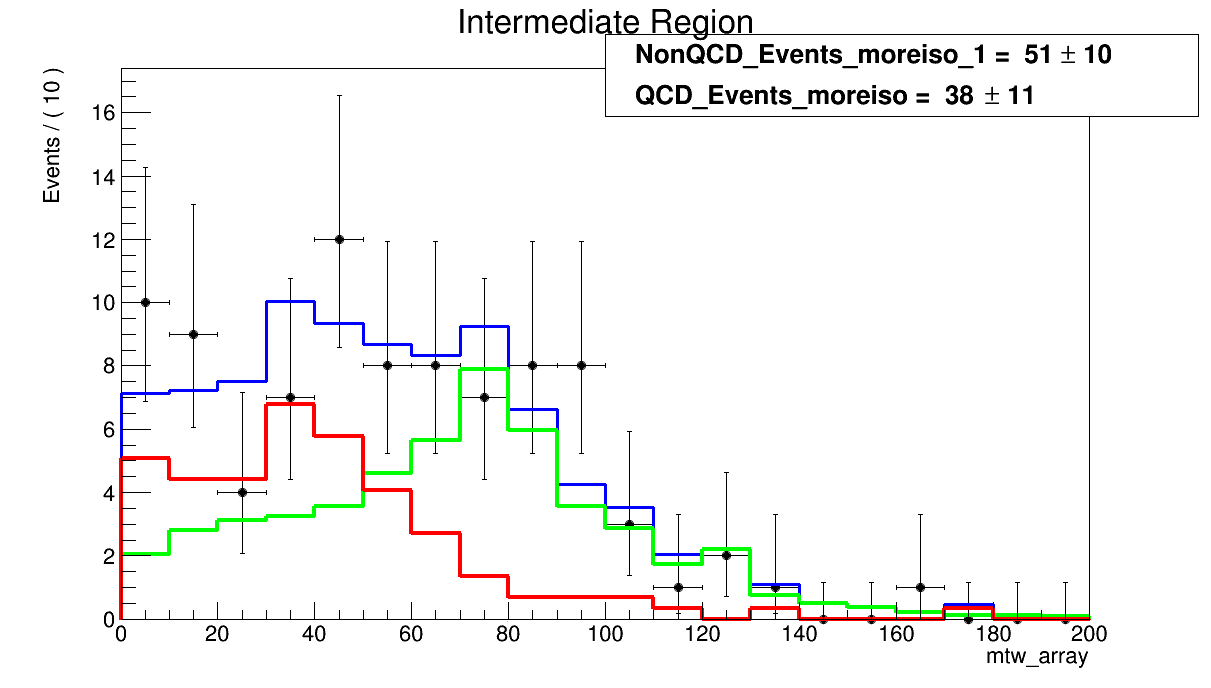
\includegraphics[scale=0.2]{figures/2J1T/MTW_fit_2j1t_moreiso_SR_NononQCDsubtraction}

\begin{centering}
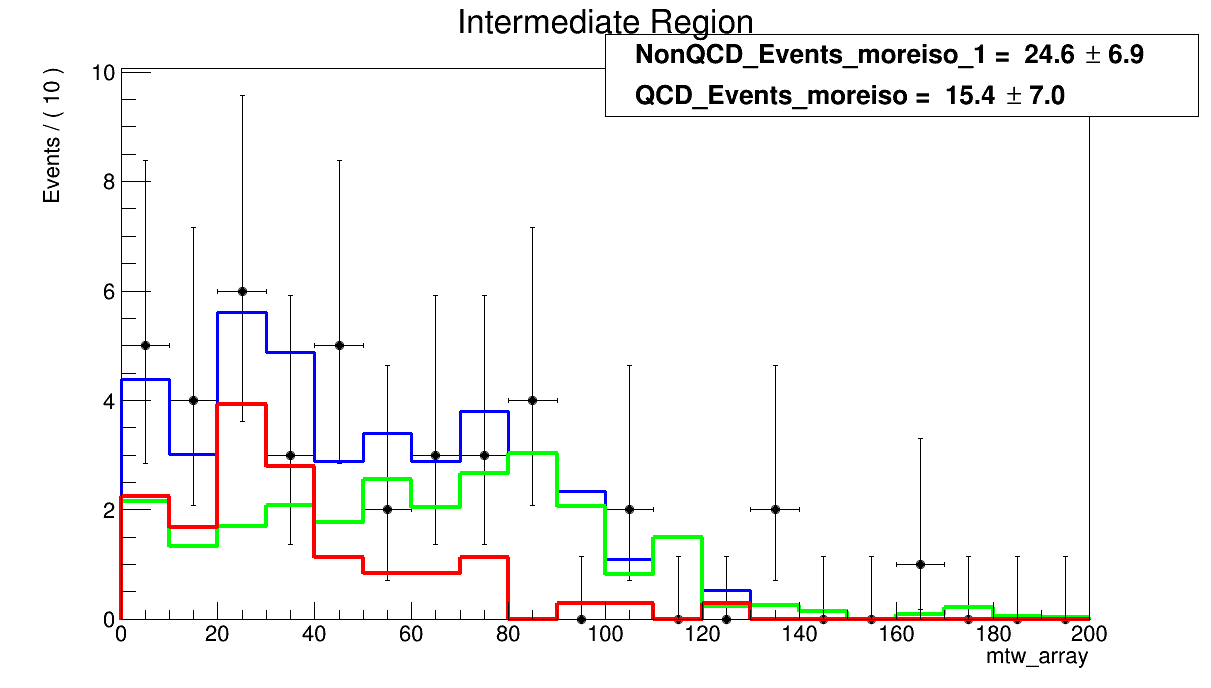
\includegraphics[scale=0.2]{figures/2J1T/MTW_fit_2j1t_moreiso_SB_NononQCDsubtraction}
\par\end{centering}
}
\caption{Fit to the ${\rm m_{T}}$ distribution in the \textquotedblleft{}2-jets
1-tag\textquotedblright{} sample inclusively (upper left), inside
(upper middle) and outside (upper right) the ${\rm m_{top}}$ window in
the signal region ($\murelIso < 0.06$). Fit to the ${\rm m_{T}}$ distribution in the
\textquotedblleft{}2-jets 1-tag\textquotedblright{} sample inclusively
(bottom left), inside (bottom middle) and outside (bottom right) the ${\rm m_{top}}$
window in the intermediate-isolated region ($0.06 < \murelIso < 0.12$). For these variations,
non QCD MC templates have not been deducted from the anti-isolated
data ($\murelIso > 0.12$).}
\end{figure}


\begin{figure}[h!]
\resizebox{ \textwidth}{!}{
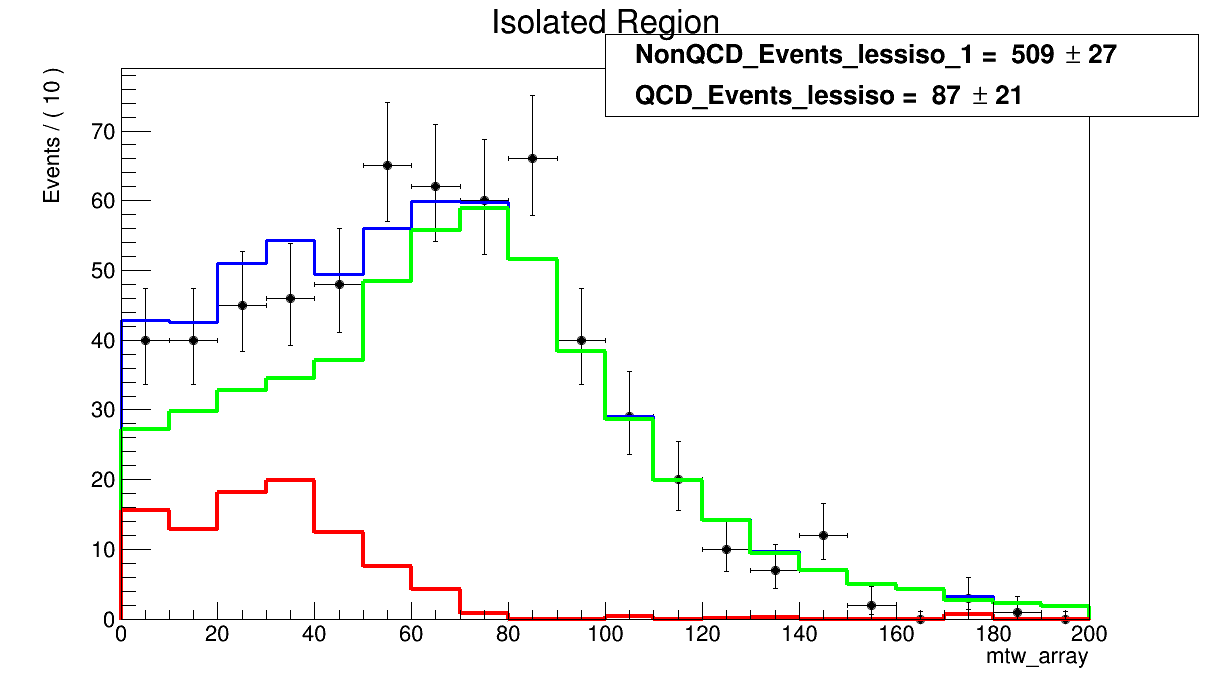
\includegraphics[scale=0.2]{figures/2J1T/MTW_fit_2j1t_lessiso_inclusive_mTop_range_nonQCDMCTemplatesScaledUp}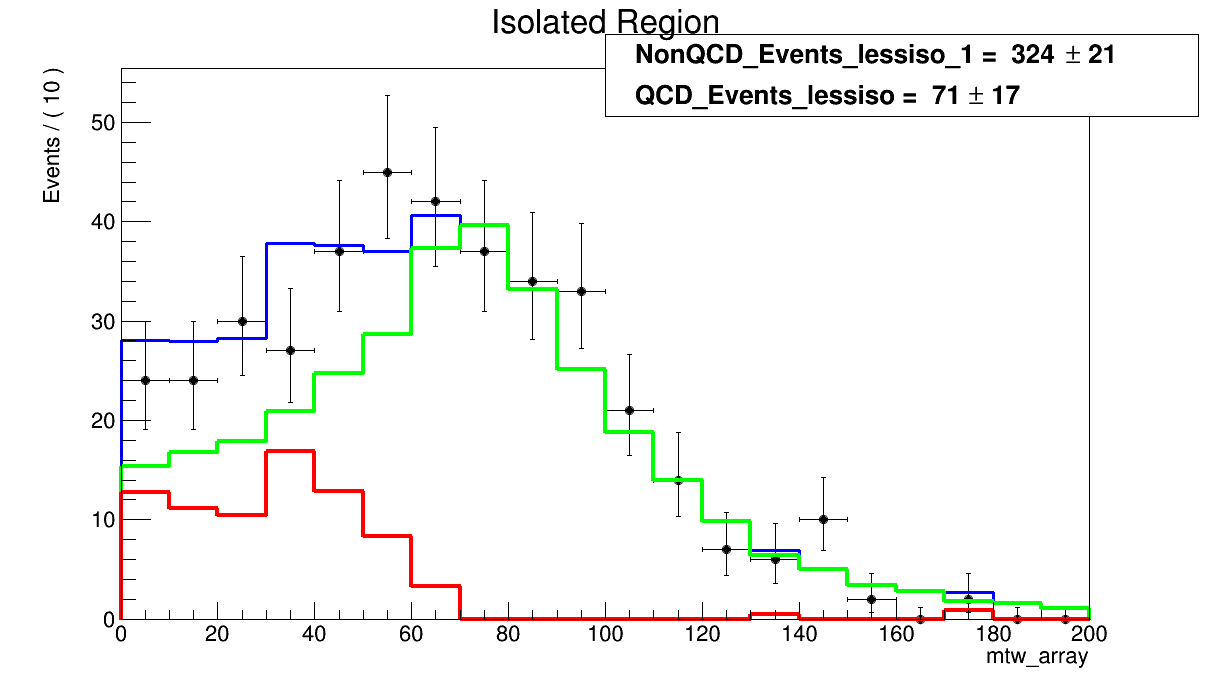
\includegraphics[scale=0.2]{figures/2J1T/MTW_fit_2j1t_lessiso_SR_nonQCDMCTemplatesScaledUp}

\begin{centering}
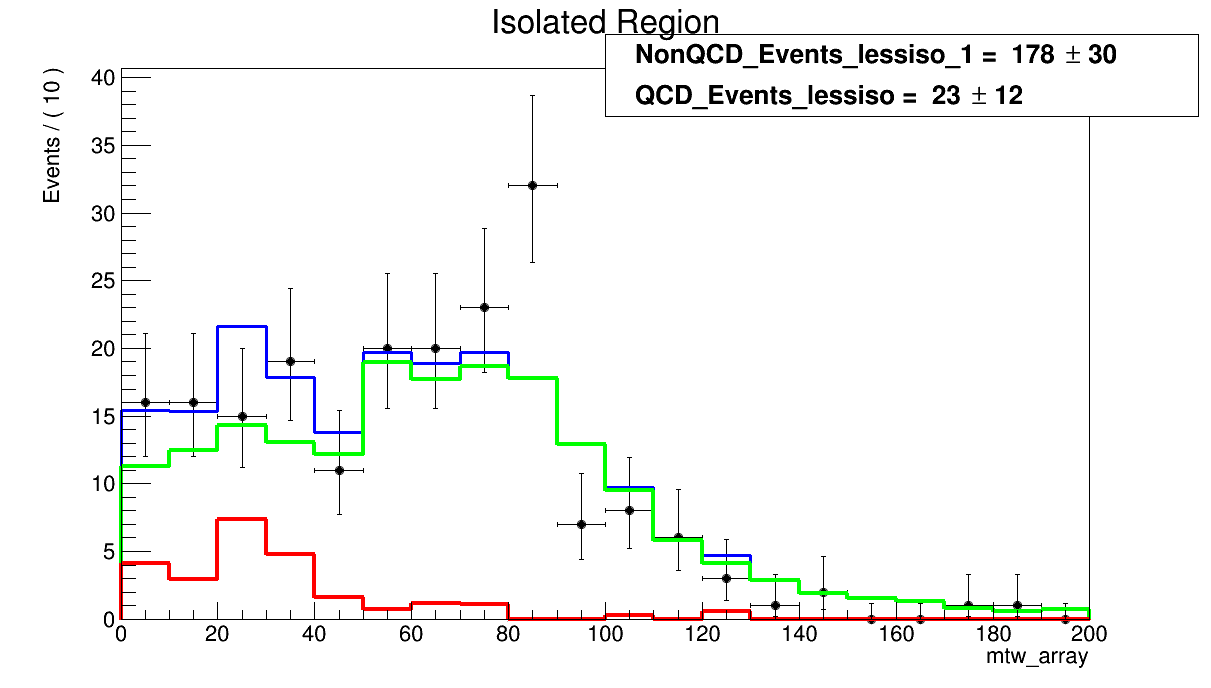
\includegraphics[scale=0.2]{figures/2J1T/MTW_fit_2j1t_lessiso_SB_nonQCDMCTemplatesScaledUp}
\par\end{centering}
}
\resizebox{ \textwidth}{!}{
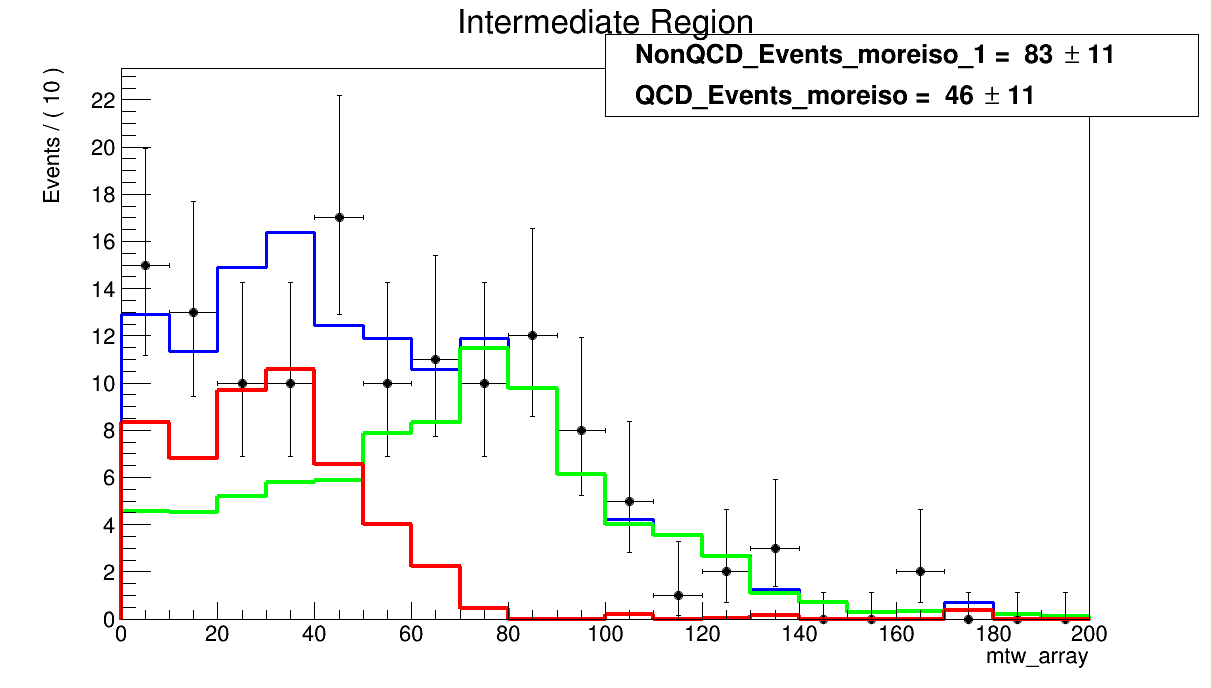
\includegraphics[scale=0.2]{figures/2J1T/MTW_fit_2j1t_moreiso_inclusive_mTop_range_nonQCDMCTemplatesScaledUp}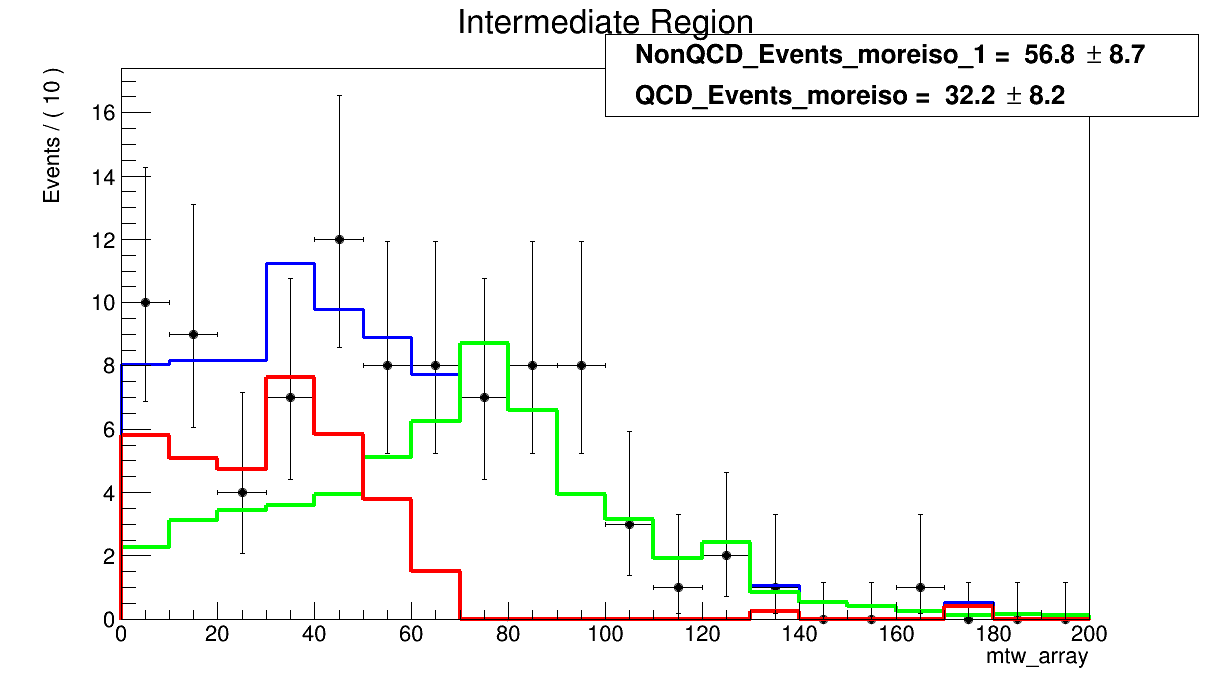
\includegraphics[scale=0.2]{figures/2J1T/MTW_fit_2j1t_moreiso_SR_nonQCDMCTemplatesScaledUp}

\begin{centering}
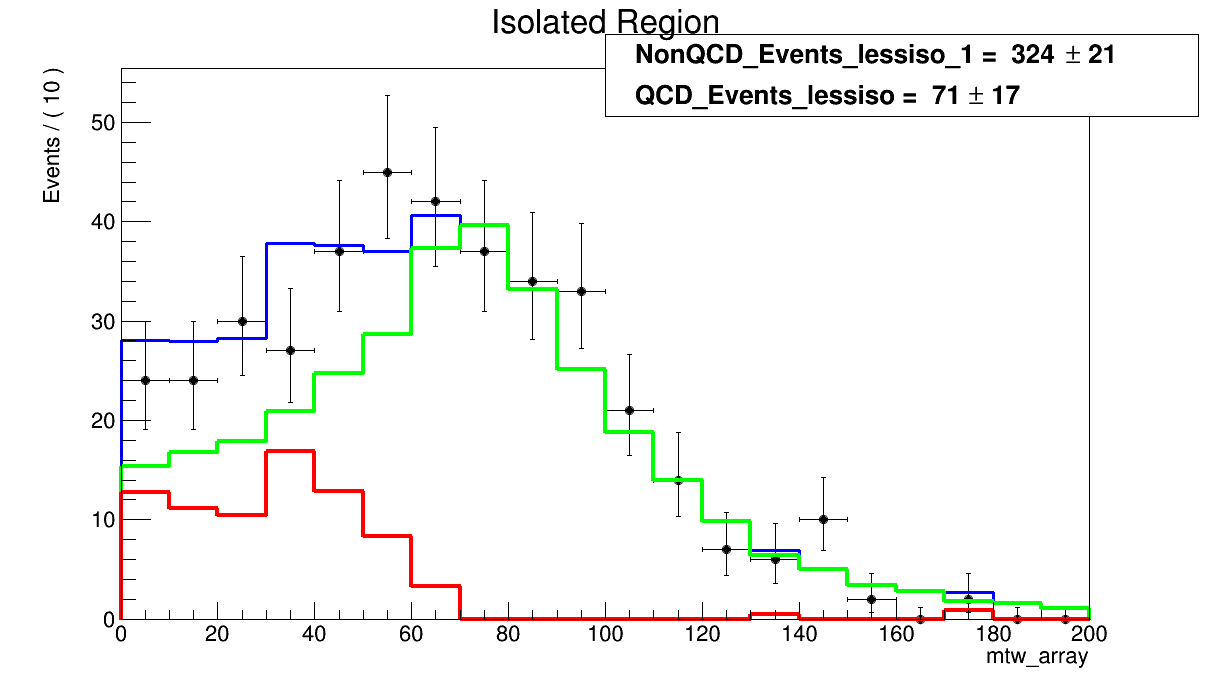
\includegraphics[scale=0.2]{figures/2J1T/MTW_fit_2j1t_lessiso_SR_nonQCDMCTemplatesScaledUp}
\par\end{centering}
}

\caption{Fit to the ${\rm m_{T}}$ distribution in the \textquotedblleft{}2-jets
1-tag\textquotedblright{} sample inclusively (upper left), inside
(upper middle) and outside (upper right) the ${\rm m_{top}}$ window in
the signal region ($\murelIso < 0.06$). Fit to the ${\rm m_{T}}$ distribution in the
\textquotedblleft{}2-jets 1-tag\textquotedblright{} sample inclusively
(bottom left), inside (bottom middle) and outside ( bottom right) the ${\rm m_{top}}$
window in the intermediate-isolated region($0.06 < \murelIso < 0.12$) . For these variations,
non QCD MC templates in the anti-isolated region ($\murelIso > 0.12$) have been scaled
up.}
\end{figure}


\begin{figure}[h!]
\resizebox{ \textwidth}{!}{
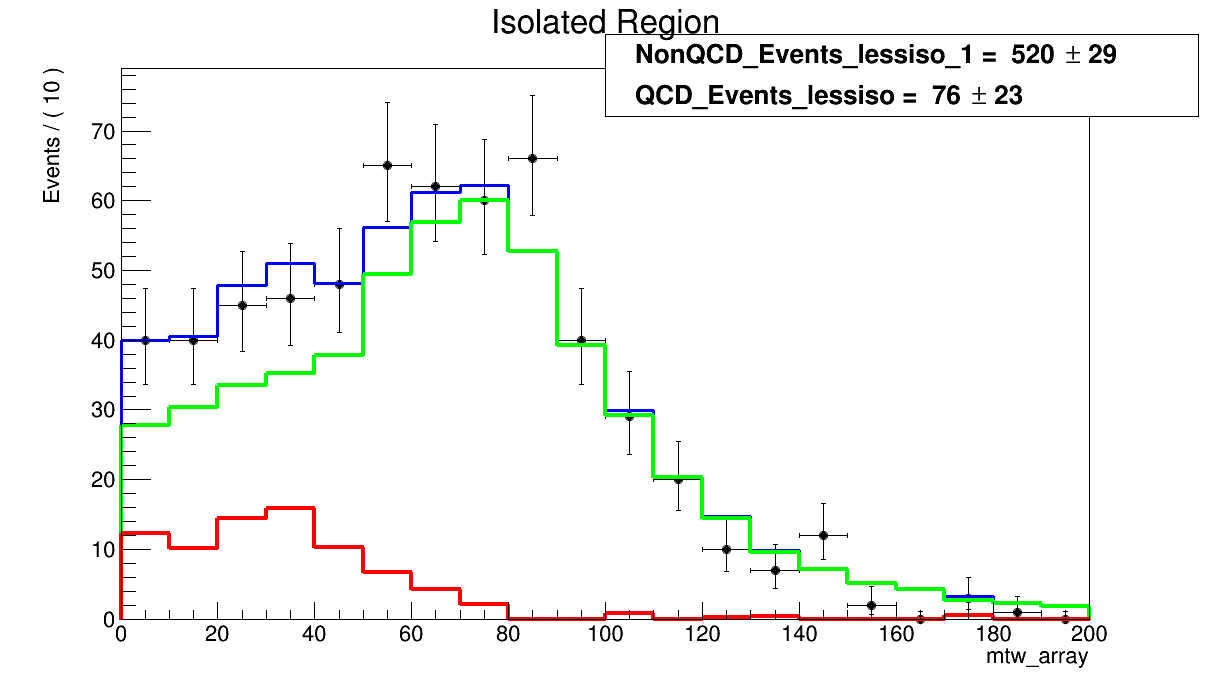
\includegraphics[scale=0.2]{figures/2J1T/MTW_fit_2j1t_lessiso_inclusive_mTop_range_nonQCDMCTemplatesScaledDown}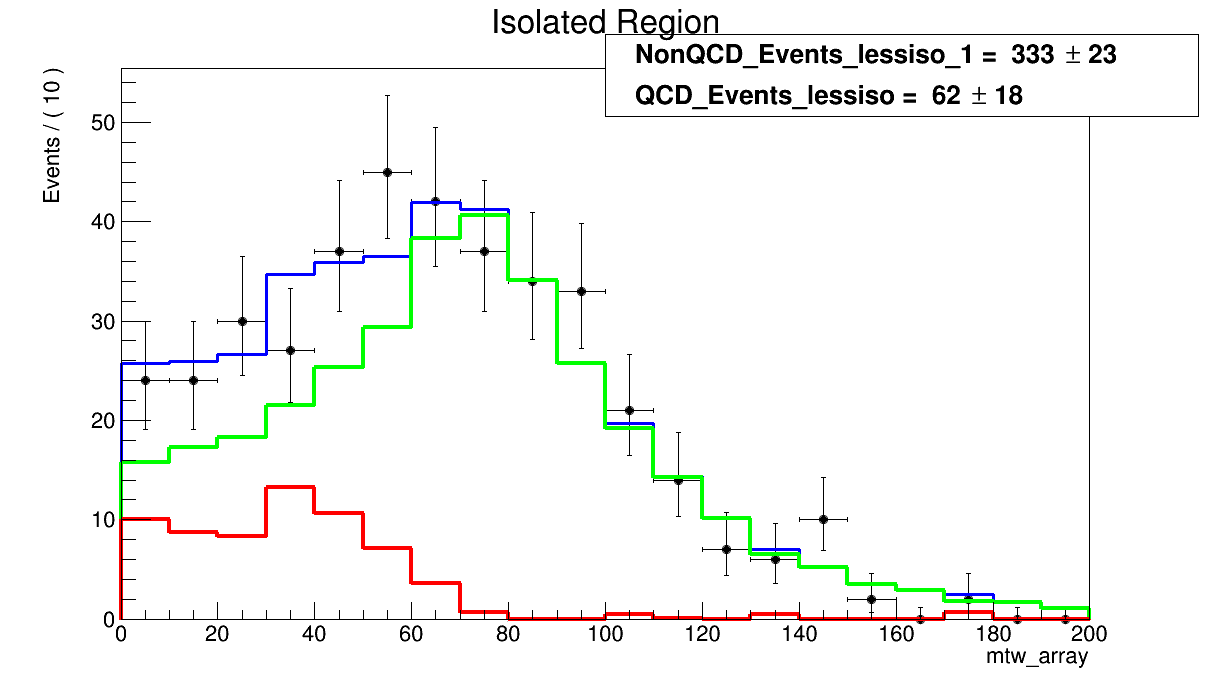
\includegraphics[scale=0.2]{figures/2J1T/MTW_fit_2j1t_lessiso_SR_nonQCDMCTemplatesScaledDown}

\begin{centering}
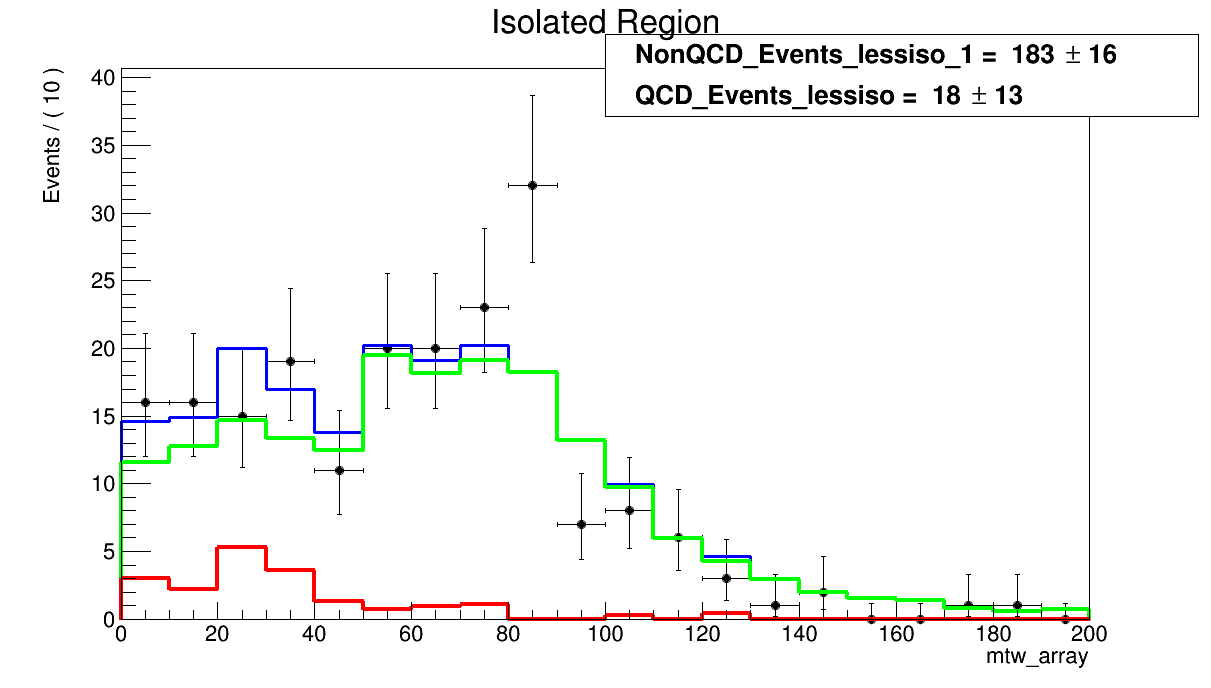
\includegraphics[scale=0.2]{figures/2J1T/MTW_fit_2j1t_lessiso_SB_nonQCDMCTemplatesScaledDown}
\par\end{centering}
}
\resizebox{ \textwidth}{!}{
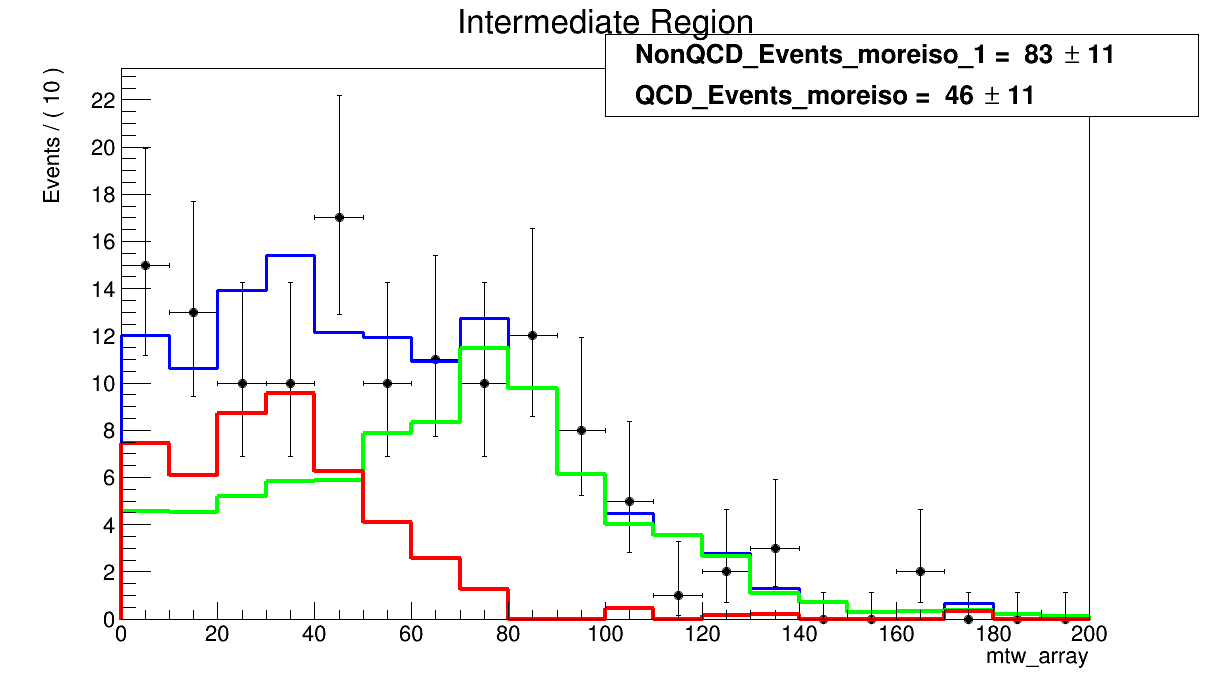
\includegraphics[scale=0.2]{figures/2J1T/MTW_fit_2j1t_moreiso_inclusive_mTop_range_nonQCDMCTemplatesScaledDown}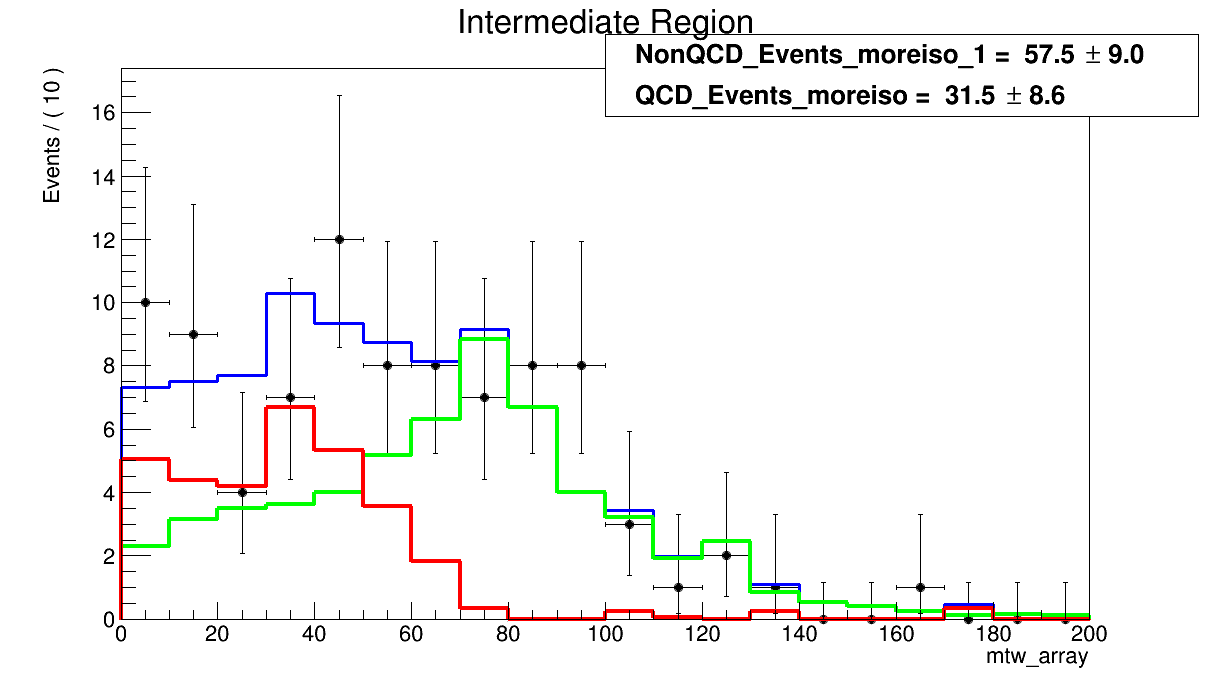
\includegraphics[scale=0.2]{figures/2J1T/MTW_fit_2j1t_moreiso_SR_nonQCDMCTemplatesScaledDown}

\begin{centering}
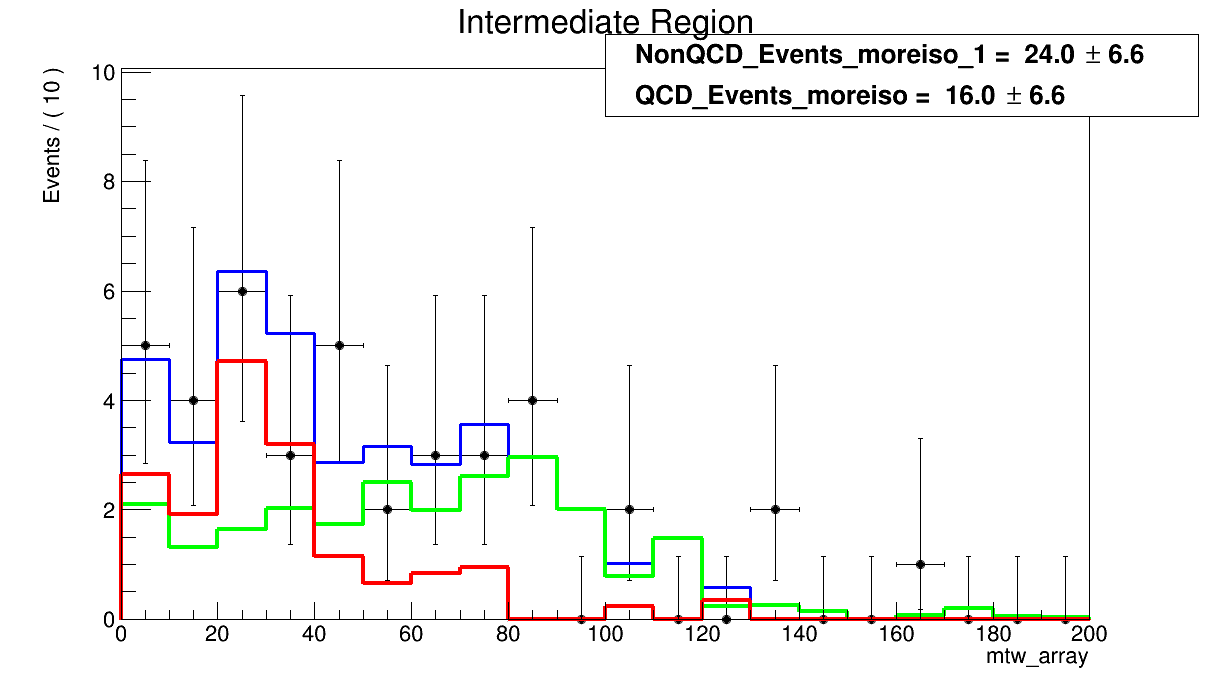
\includegraphics[scale=0.2]{figures/2J1T/MTW_fit_2j1t_moreiso_SB_nonQCDMCTemplatesScaledDown}
\par\end{centering}
}
\caption{Fit to the ${\rm m_{T}}$ distribution in the \textquotedblleft{}2-jets
1-tag\textquotedblright{} sample inclusively (upper left), inside
(upper middle) and outside (upper right) the ${\rm m_{top}}$ window in
the signal region ($\murelIso < 0.06$). Fit to the ${\rm m_{T}}$ distribution in the
\textquotedblleft{}2-jets 1-tag\textquotedblright{} sample inclusively
(bottom left), inside (bottom middle) and outside ( bottom right) the ${\rm m_{top}}$
window in the intermediate-isolated region ($0.06 < \murelIso < 0.12$). For these variations,
non QCD MC templates in the anti-isolated region ($\murelIso > 0.12$) have been scaled
down.}
\end{figure}

\clearpage

\subsection{Fit in a $\mT$ sub-range}

\begin{figure}[h!]
\resizebox{ \textwidth}{!}{
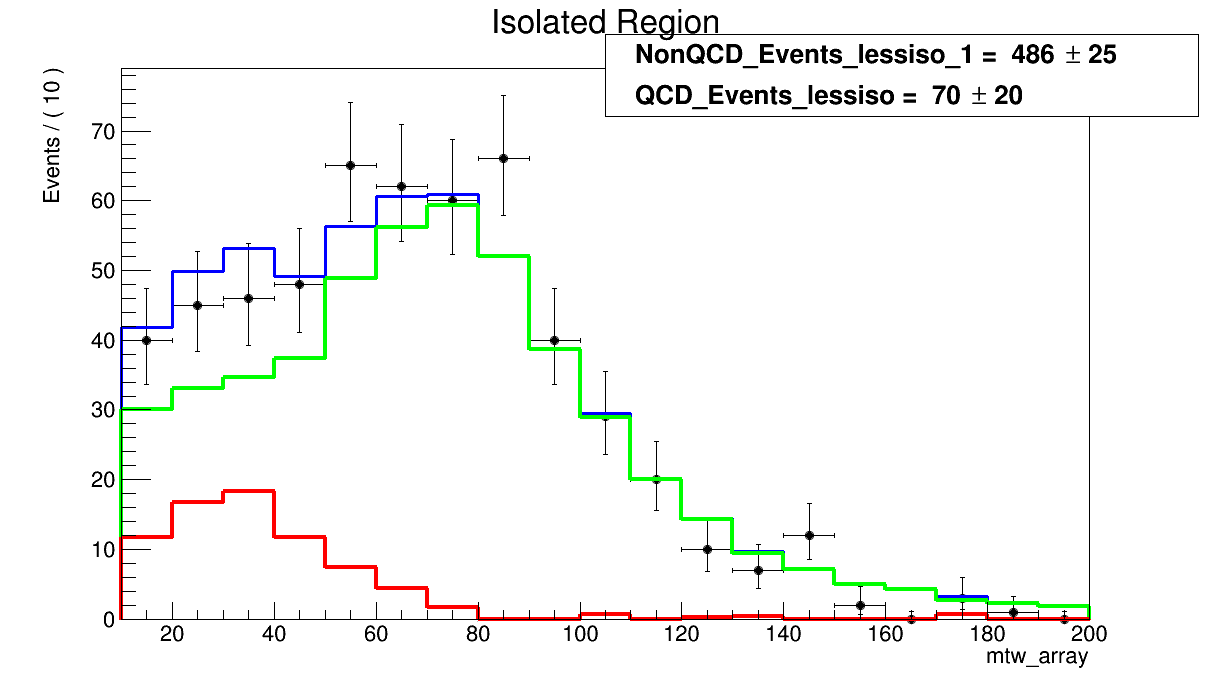
\includegraphics[scale=0.2]{figures/2J1T/MTW_fit_2j1t_lessiso_inclusive_mTop_range_GreaterThan10}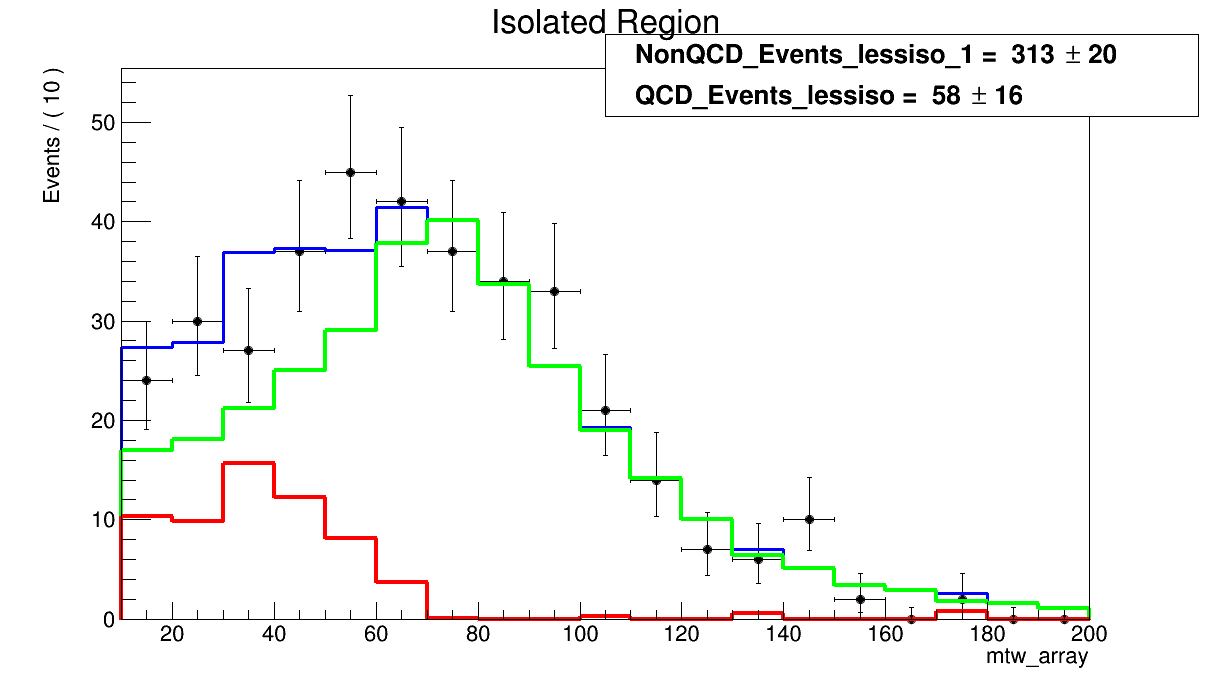
\includegraphics[scale=0.2]{figures/2J1T/MTW_fit_2j1t_lessiso_SR_GreaterThan10}

\begin{centering}
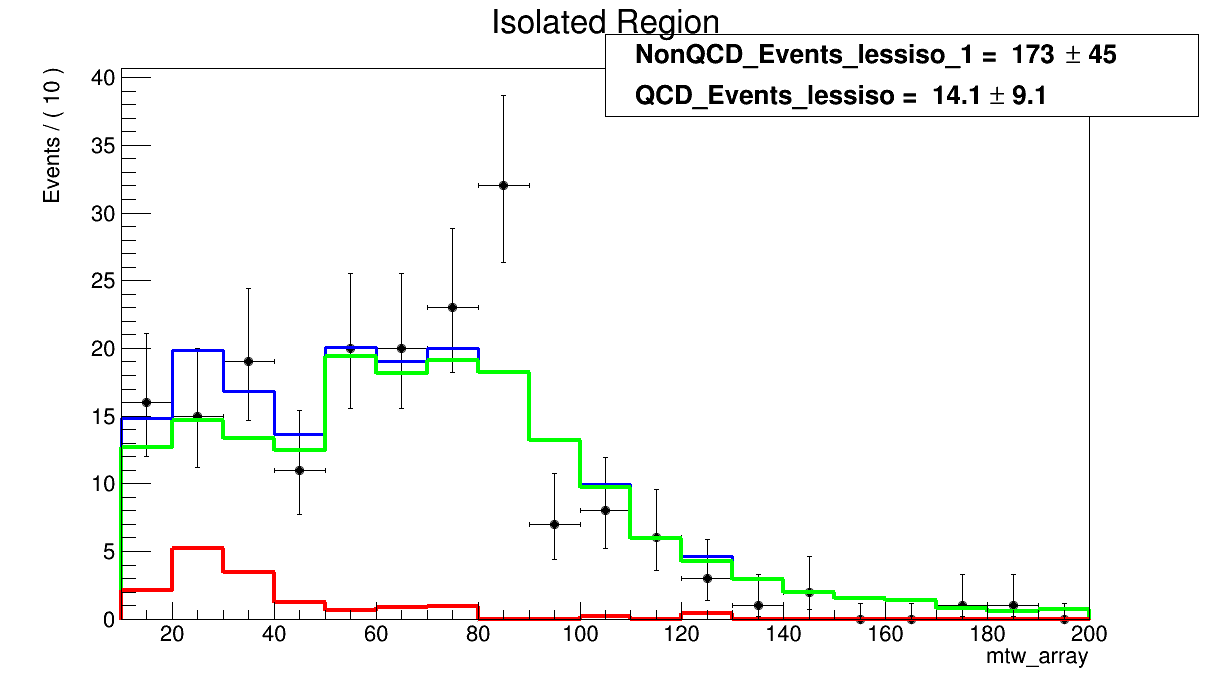
\includegraphics[scale=0.2]{figures/2J1T/MTW_fit_2j1t_lessiso_SB_GreaterThan10}
\par\end{centering}
}
\resizebox{ \textwidth}{!}{
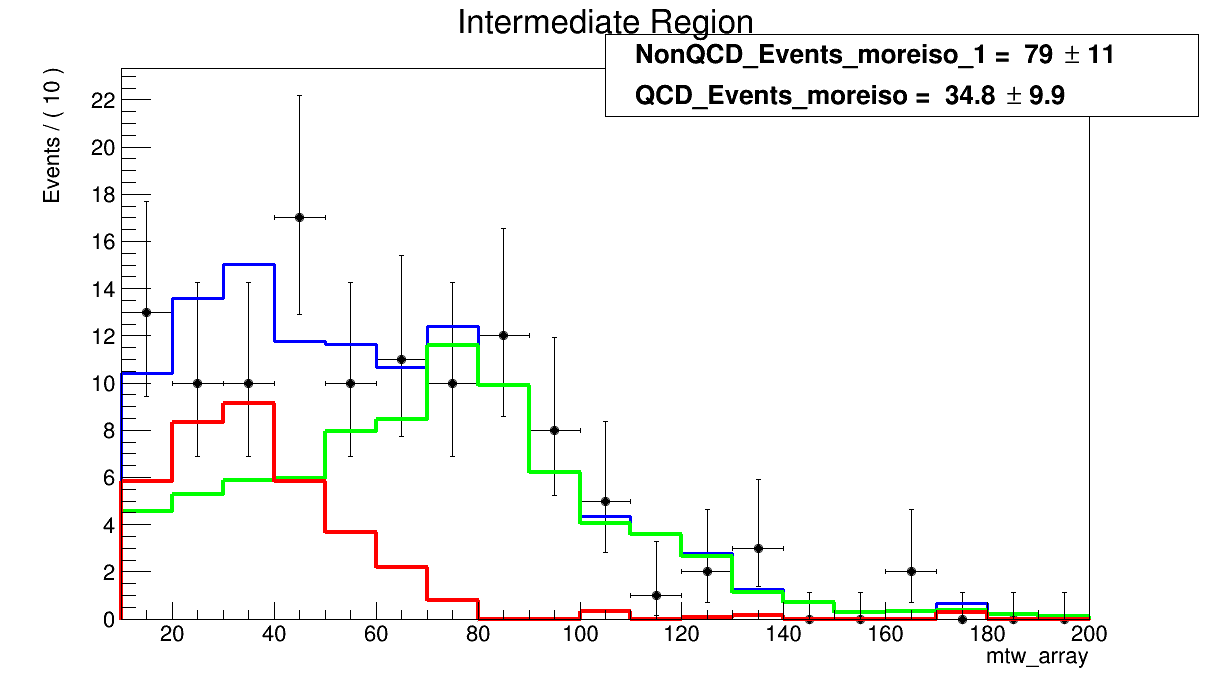
\includegraphics[scale=0.2]{figures/2J1T/MTW_fit_2j1t_moreiso_inclusive_mTop_range_GreaterThan10}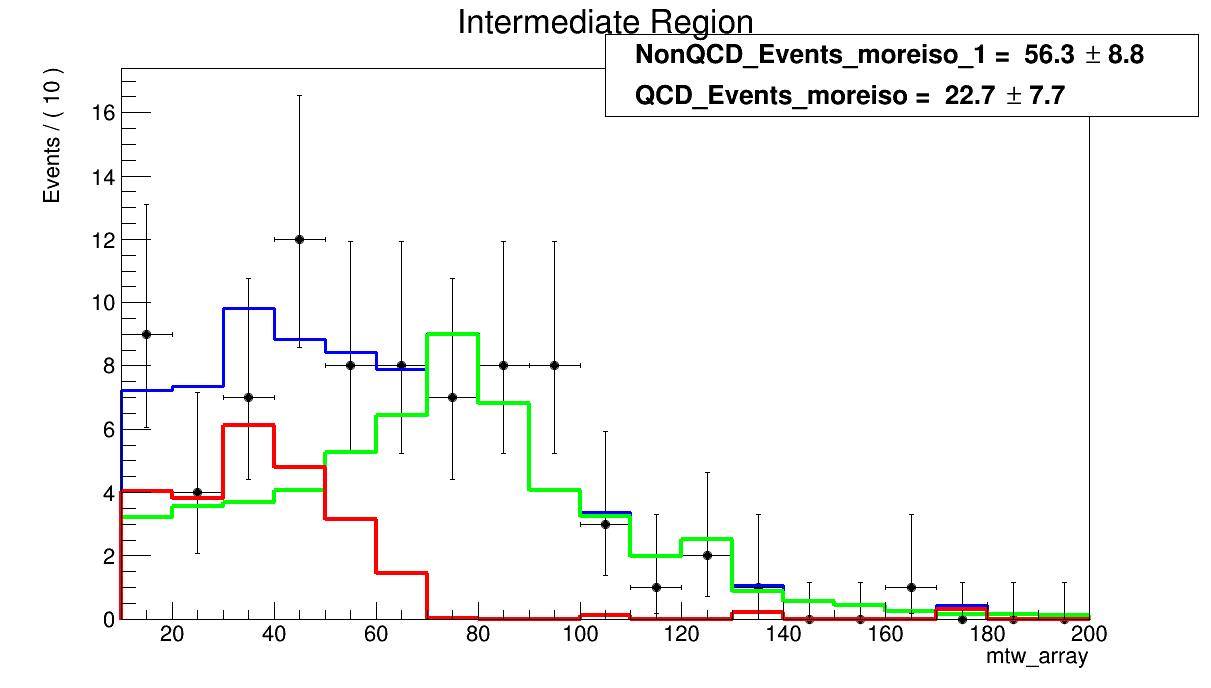
\includegraphics[scale=0.2]{figures/2J1T/MTW_fit_2j1t_moreiso_SR_GreaterThan10}

\begin{centering}
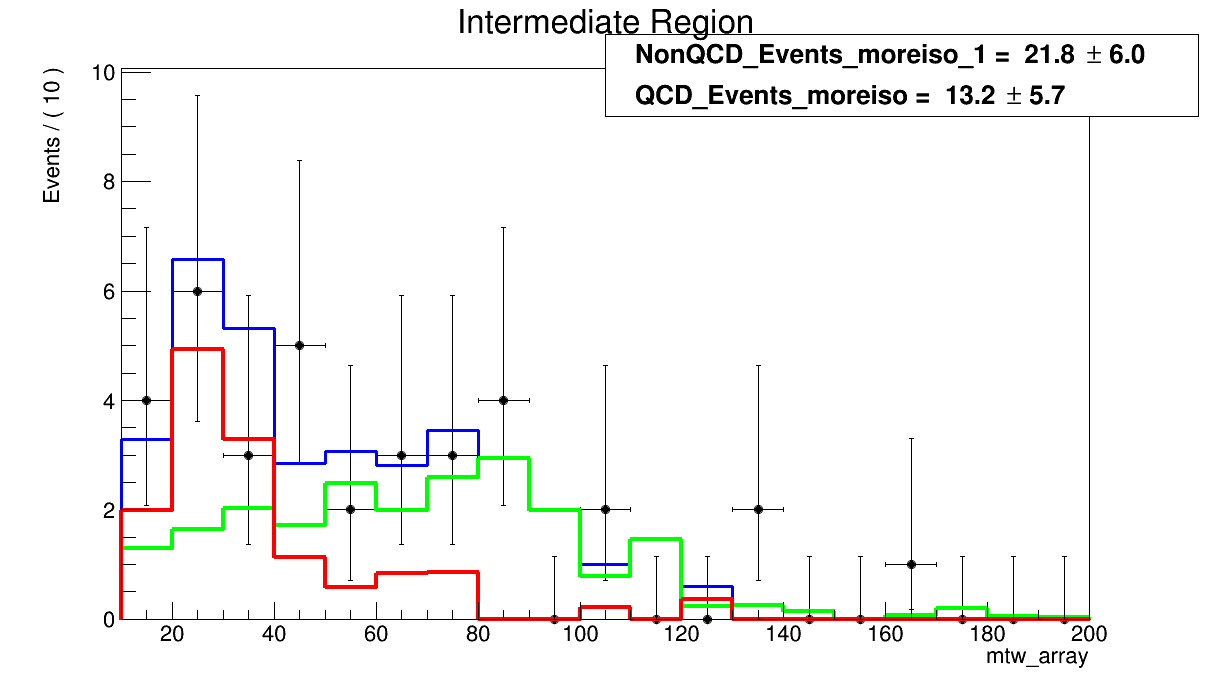
\includegraphics[scale=0.2]{figures/2J1T/MTW_fit_2j1t_moreiso_SB_GreaterThan10}
\par\end{centering}
}
\caption{Fit to the ${\rm m_{T}}$ distribution in the \textquotedblleft{}2-jets
1-tag\textquotedblright{} sample inclusively (upper left), inside
(upper middle) and outside (upper right) the ${\rm m_{top}}$ window in
the signal region ($\murelIso < 0.06$). Fit to the ${\rm m_{T}}$ distribution in the
\textquotedblleft{}2-jets 1-tag\textquotedblright{} sample inclusively
(bottom left), inside (bottom middle) and outside (bottom right) the ${\rm m_{top}}$
window in the intermediate-isolated region ($0.06 < \murelIso < 0.12$). }
\end{figure}

\clearpage

\subsection{Fit with more nonQCD components}

\begin{figure}[h!]
\resizebox{ \textwidth}{!}{
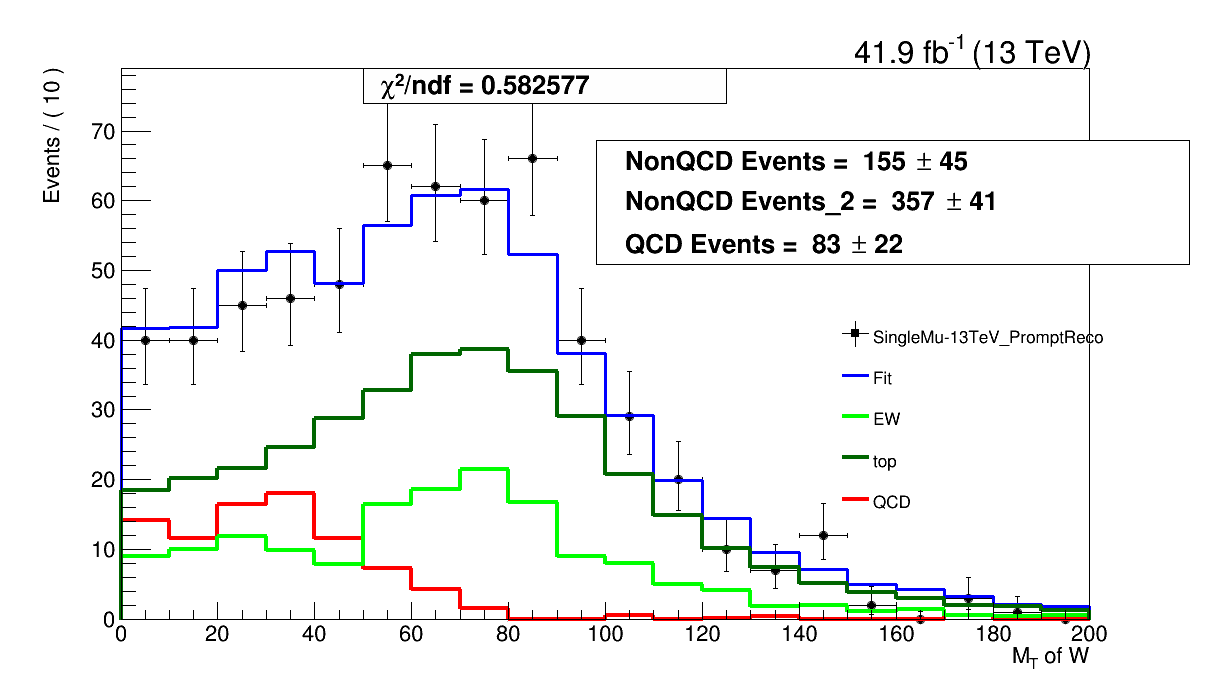
\includegraphics[scale=0.2]{figures/2J1T/MTW_fit_2j1t_lessiso_inclusive_mTop_range_threenonQCDtemplates}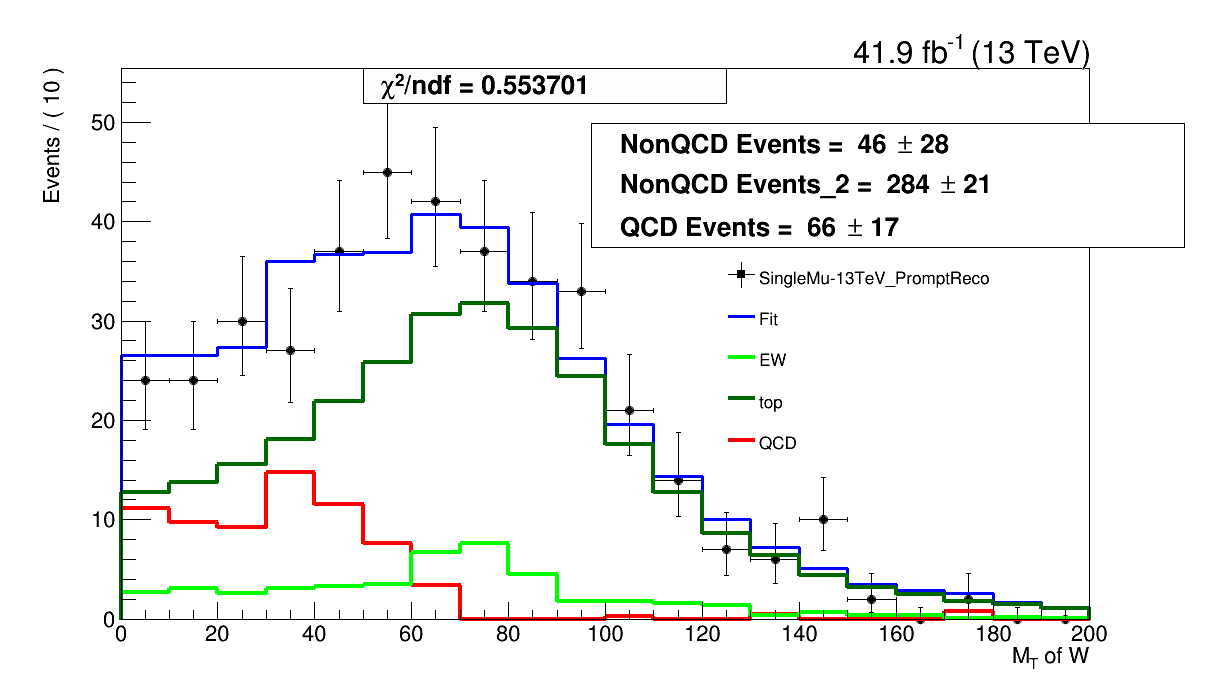
\includegraphics[scale=0.2]{figures/2J1T/MTW_fit_2j1t_lessiso_SR_threenonQCDtemplates}

\begin{centering}
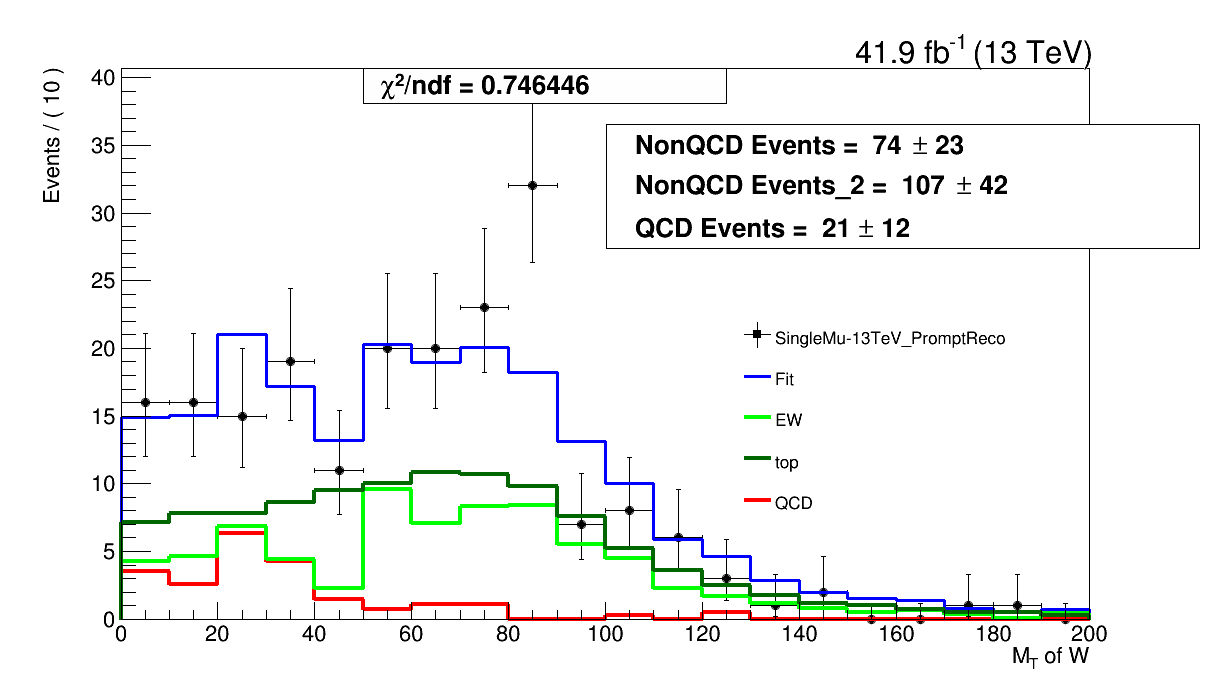
\includegraphics[scale=0.2]{figures/2J1T/MTW_fit_2j1t_lessiso_SB_threenonQCDtemplates}
\par\end{centering}
}
\resizebox{ \textwidth}{!}{
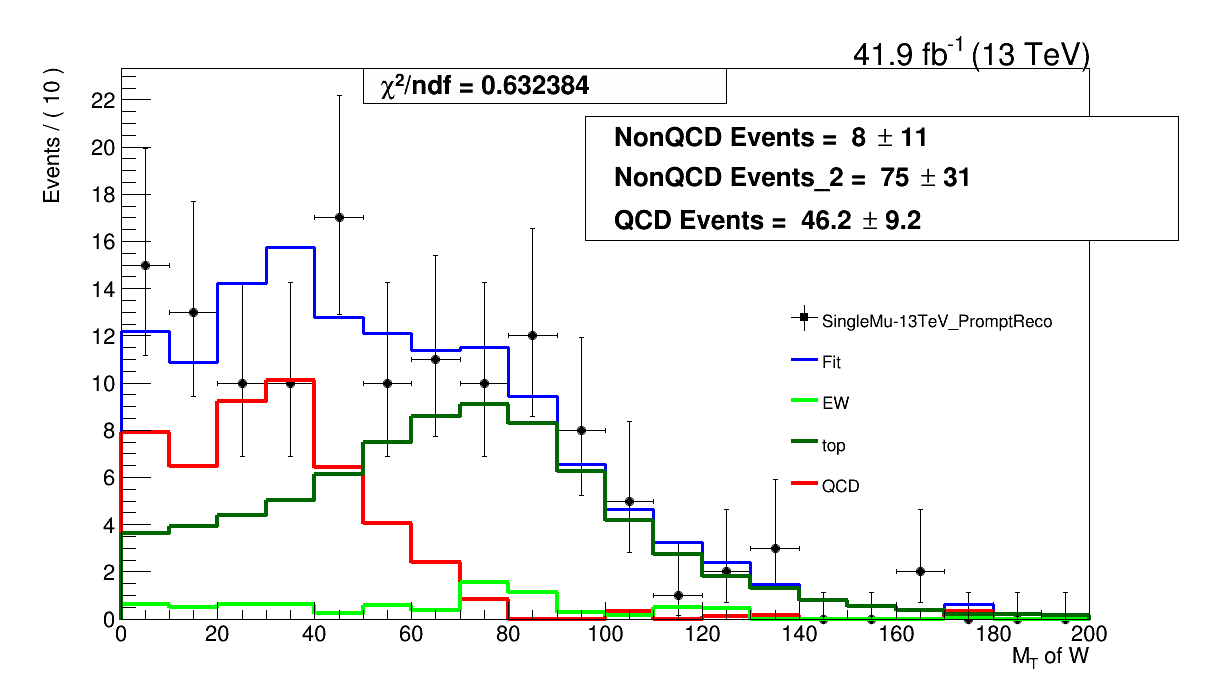
\includegraphics[scale=0.2]{figures/2J1T/MTW_fit_2j1t_moreiso_inclusive_mTop_range_threenonQCDtemplates}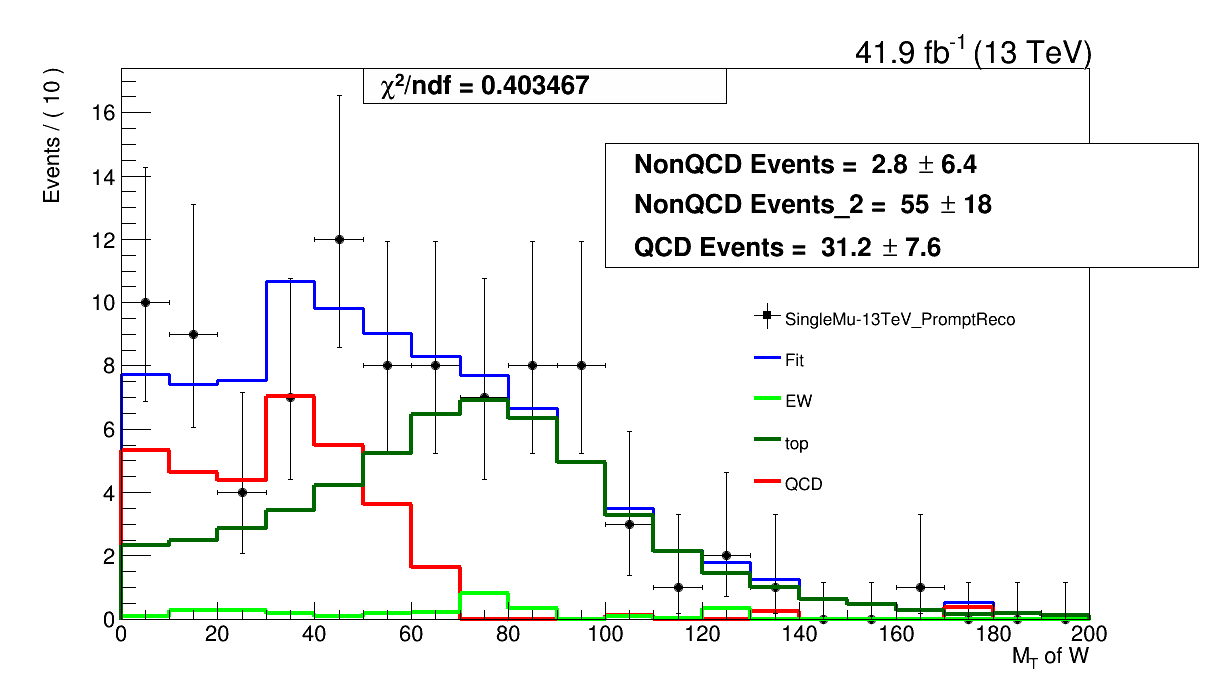
\includegraphics[scale=0.2]{figures/2J1T/MTW_fit_2j1t_moreiso_SR_threenonQCDtemplates}

\begin{centering}
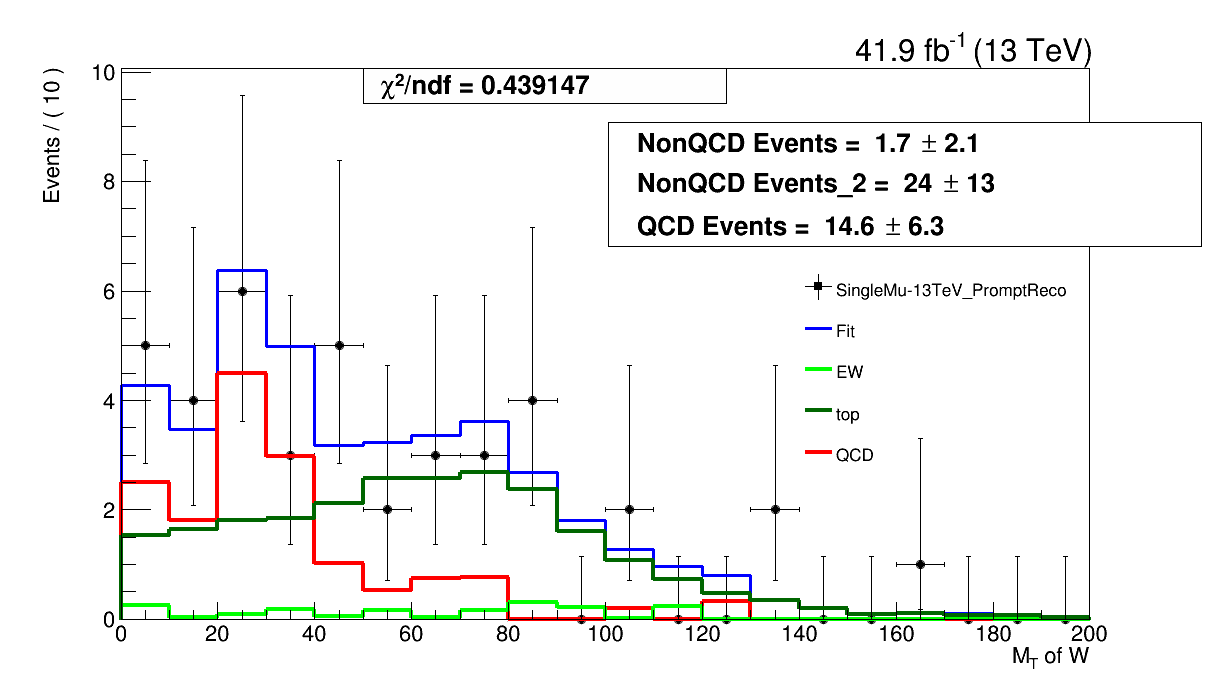
\includegraphics[scale=0.2]{figures/2J1T/MTW_fit_2j1t_moreiso_SB_threenonQCDtemplates}
\par\end{centering}
}
\caption{Fit to the ${\rm m_{T}}$ distribution in the \textquotedblleft{}2-jets
1-tag\textquotedblright{} sample inclusively (upper left), inside
(upper middle) and outside (upper right) the ${\rm m_{top}}$ window in
the signal region ($\murelIso < 0.06$). Fit to the ${\rm m_{T}}$ distribution in the
\textquotedblleft{}2-jets 1-tag\textquotedblright{} sample inclusively
(bottom left), inside (bottom middle) and outside (bottom right) the ${\rm m_{top}}$
window in the intermediate-isolated region ($0.06 < \murelIso < 0.12$). }
\end{figure}

\clearpage

\subsection{Fit with the MC template}

\begin{figure}[h!]
\resizebox{ \textwidth}{!}{
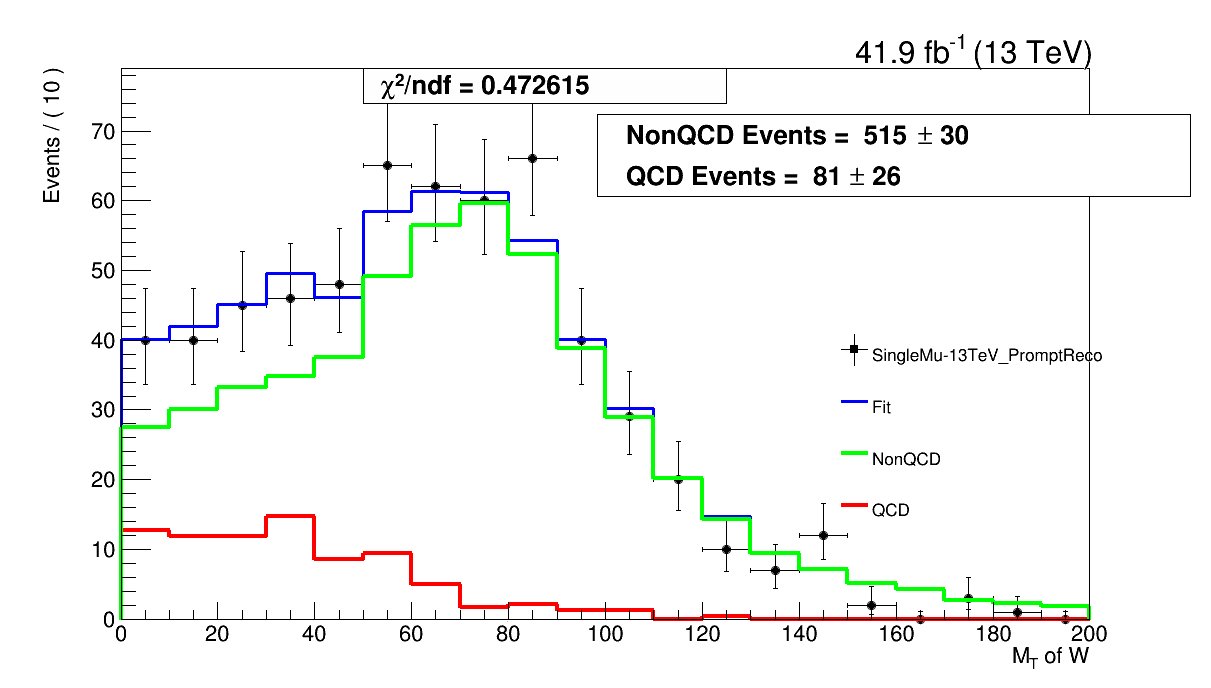
\includegraphics[scale=0.2]{figures/2J1T/MTW_fit_2j1t_lessiso_inclusive_mTop_range_MCnonQCDtemplate}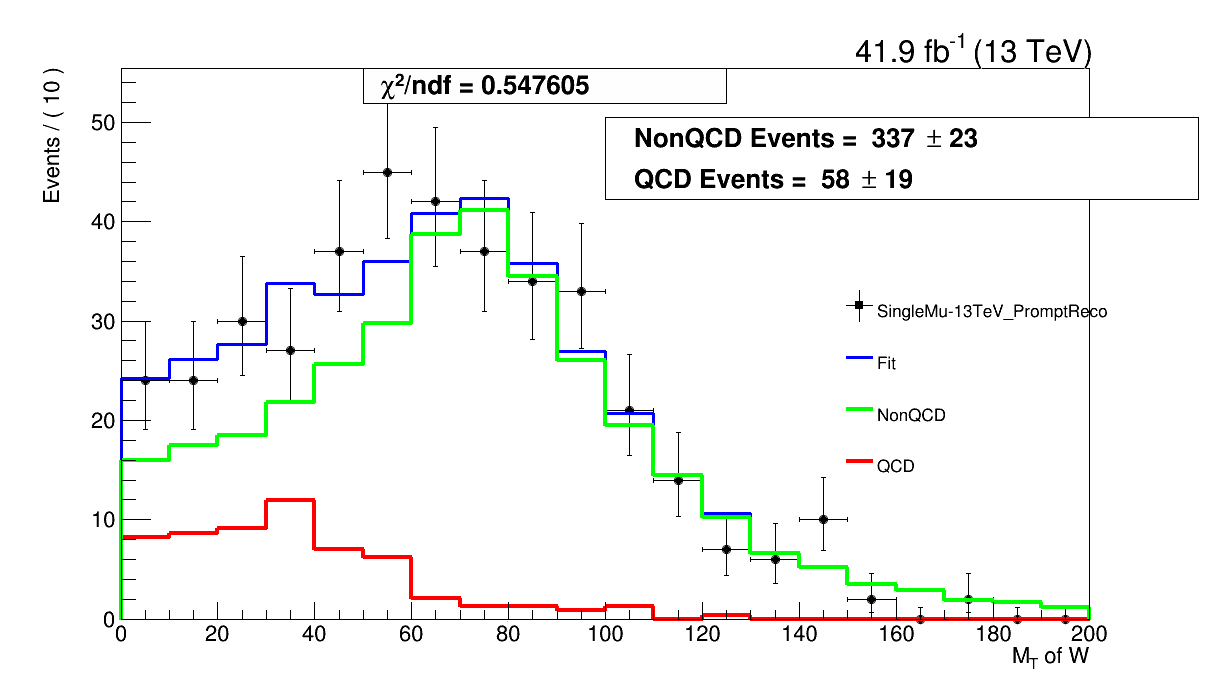
\includegraphics[scale=0.2]{figures/2J1T/MTW_fit_2j1t_lessiso_SR_MCnonQCDtemplate}

\begin{centering}
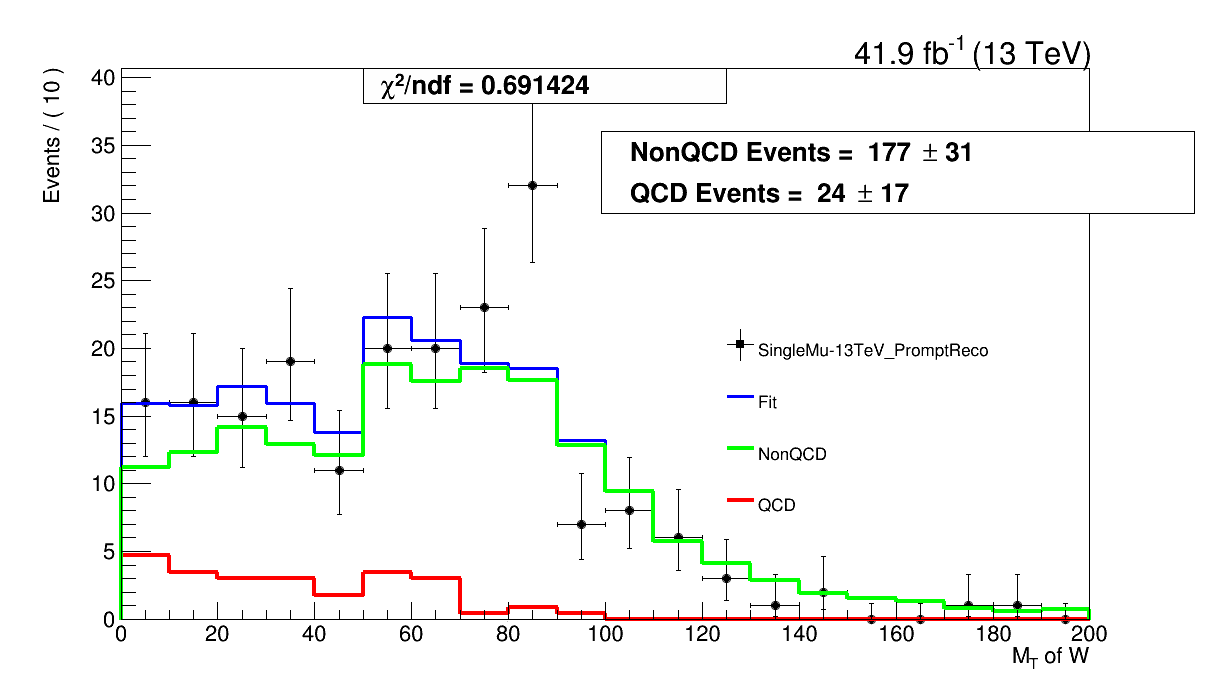
\includegraphics[scale=0.2]{figures/2J1T/MTW_fit_2j1t_lessiso_SB_MCnonQCDtemplate}
\par\end{centering}
}
\resizebox{ \textwidth}{!}{
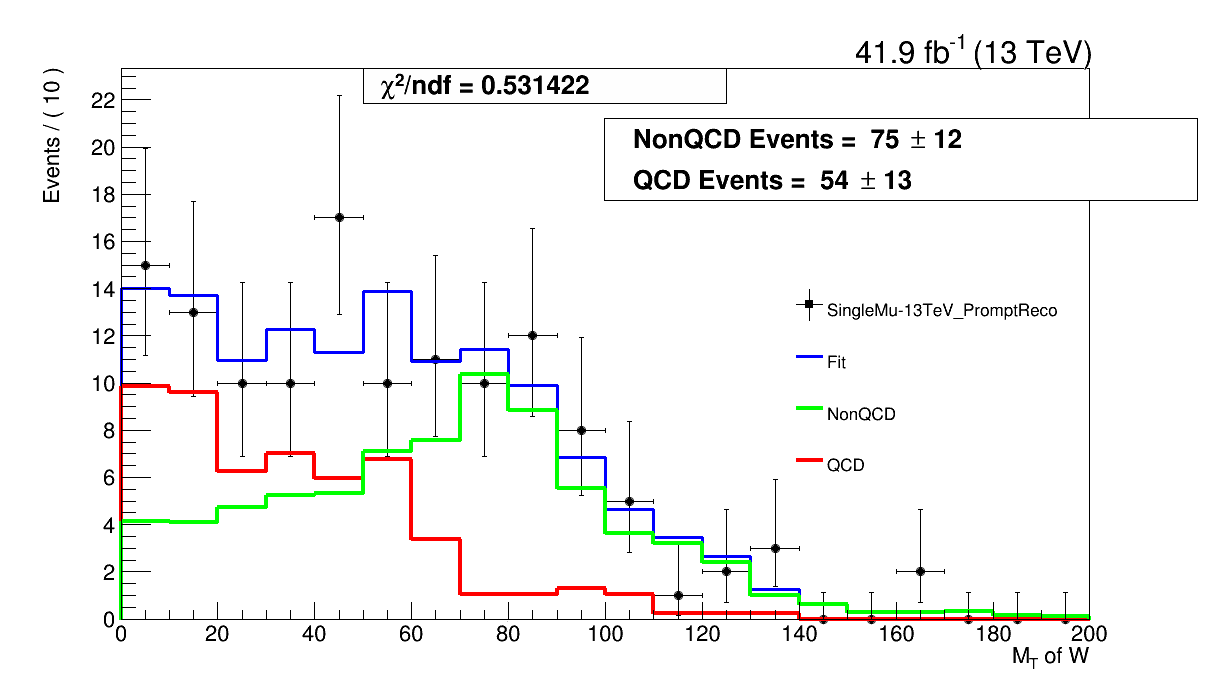
\includegraphics[scale=0.2]{figures/2J1T/MTW_fit_2j1t_moreiso_inclusive_mTop_range_MCnonQCDtemplate}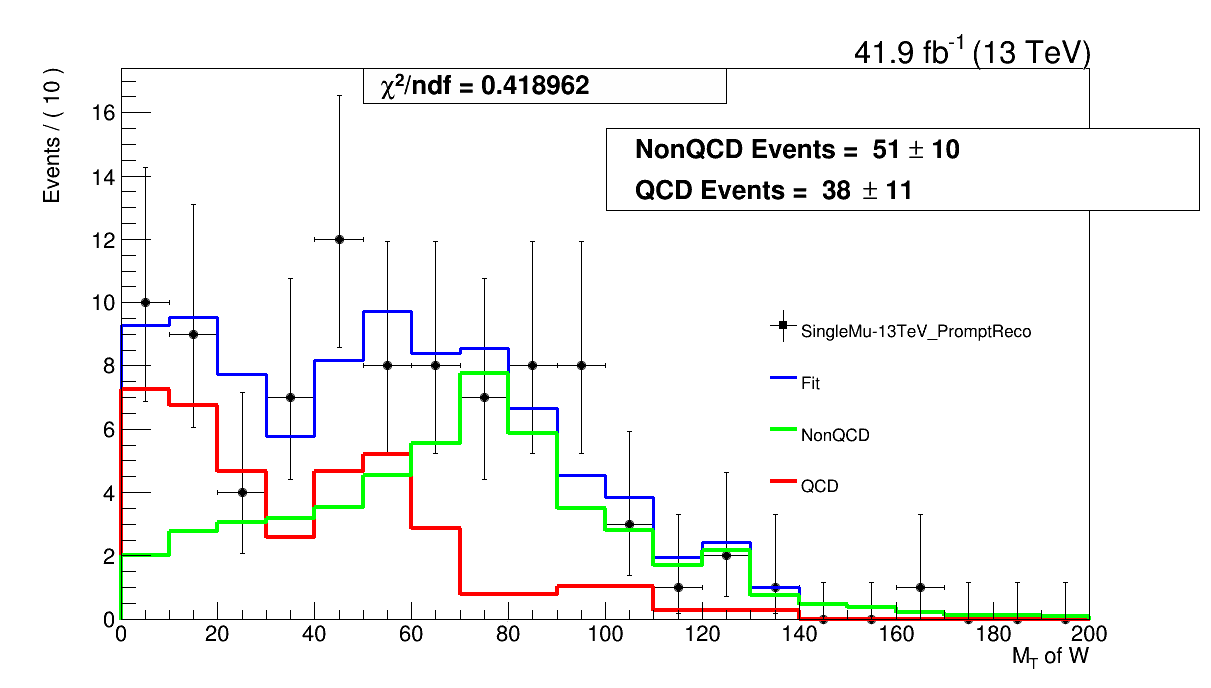
\includegraphics[scale=0.2]{figures/2J1T/MTW_fit_2j1t_moreiso_SR_MCnonQCDtemplate}

\begin{centering}
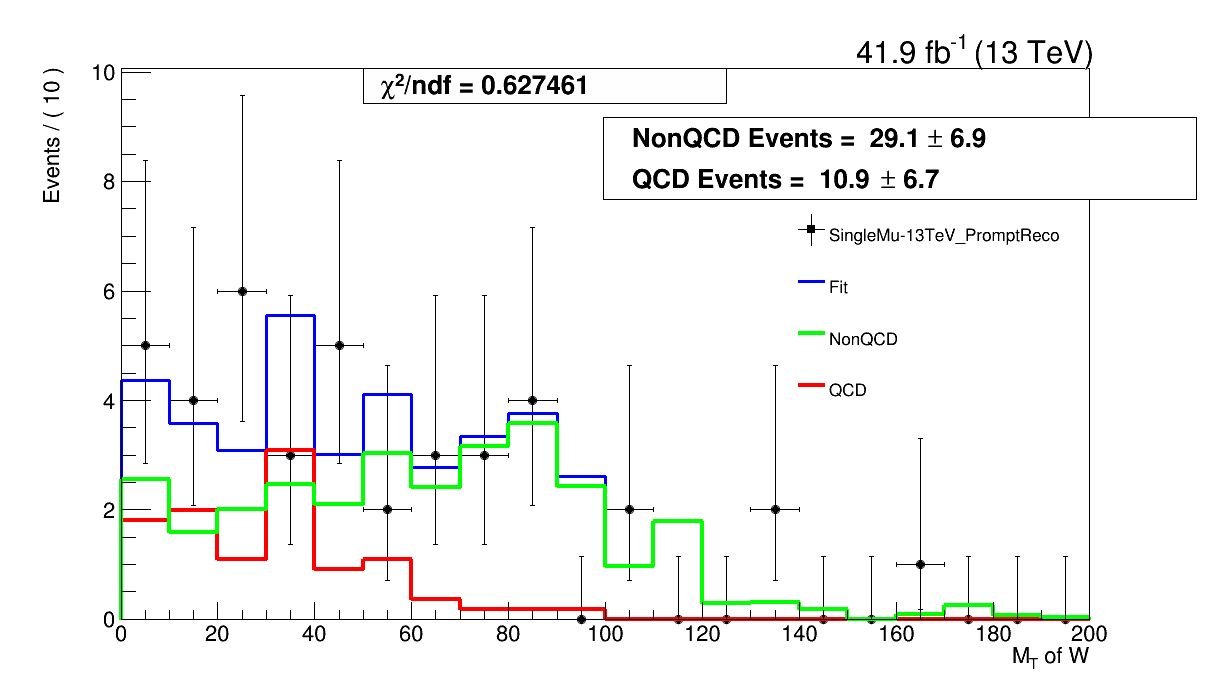
\includegraphics[scale=0.2]{figures/2J1T/MTW_fit_2j1t_moreiso_SB_MCnonQCDtemplate}
\par\end{centering}
}
\caption{Fit to the ${\rm m_{T}}$ distribution in the \textquotedblleft{}2-jets
1-tag\textquotedblright{} sample inclusively (upper left), inside
(upper middle) and outside (upper right) the ${\rm m_{top}}$ window in
the signal region. Fit to the ${\rm m_{T}}$ distribution in the
\textquotedblleft{}2-jets 1-tag\textquotedblright{} sample inclusively
(bottom left), inside (bottom middle) and outside (bottom right) the ${\rm m_{top}}$
window in the intermediate-isolated region ($0.06 < \murelIso < 0.12$). }
\end{figure}

\clearpage

\subsection{Fit using $\met$ template}

\begin{figure}[h!]
\resizebox{ \textwidth}{!}{
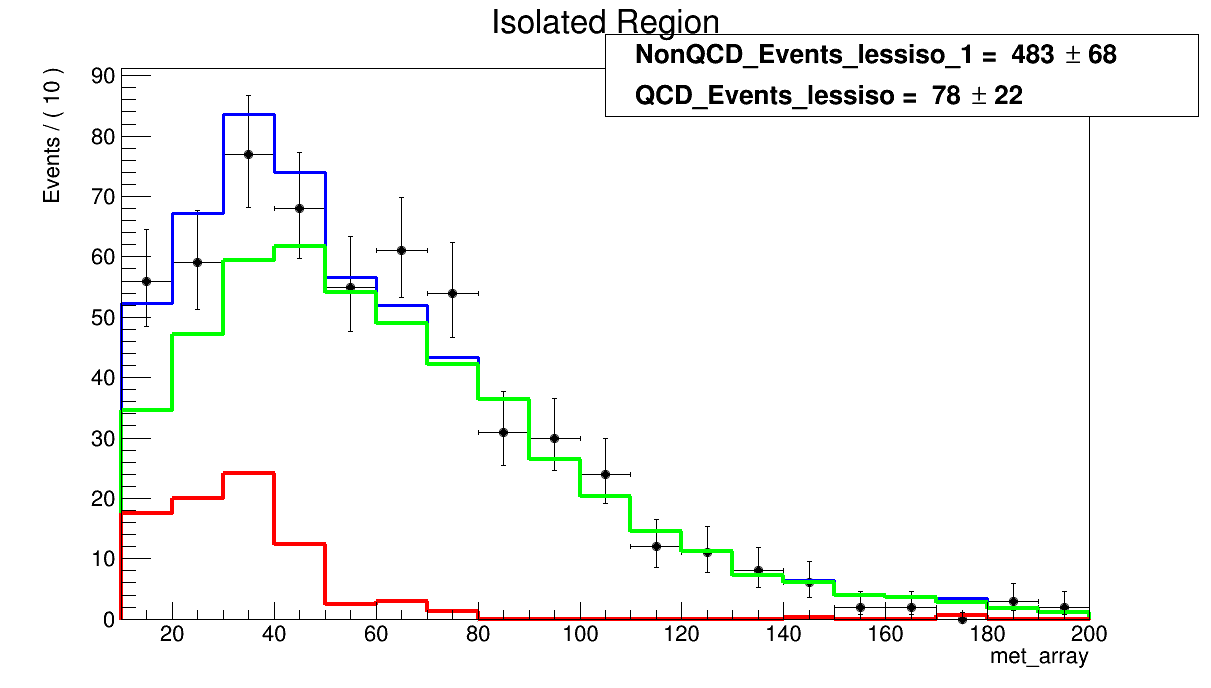
\includegraphics[scale=0.2]{figures/2J1T/MET_fit_2j1t_lessiso_inclusive_mTop_range}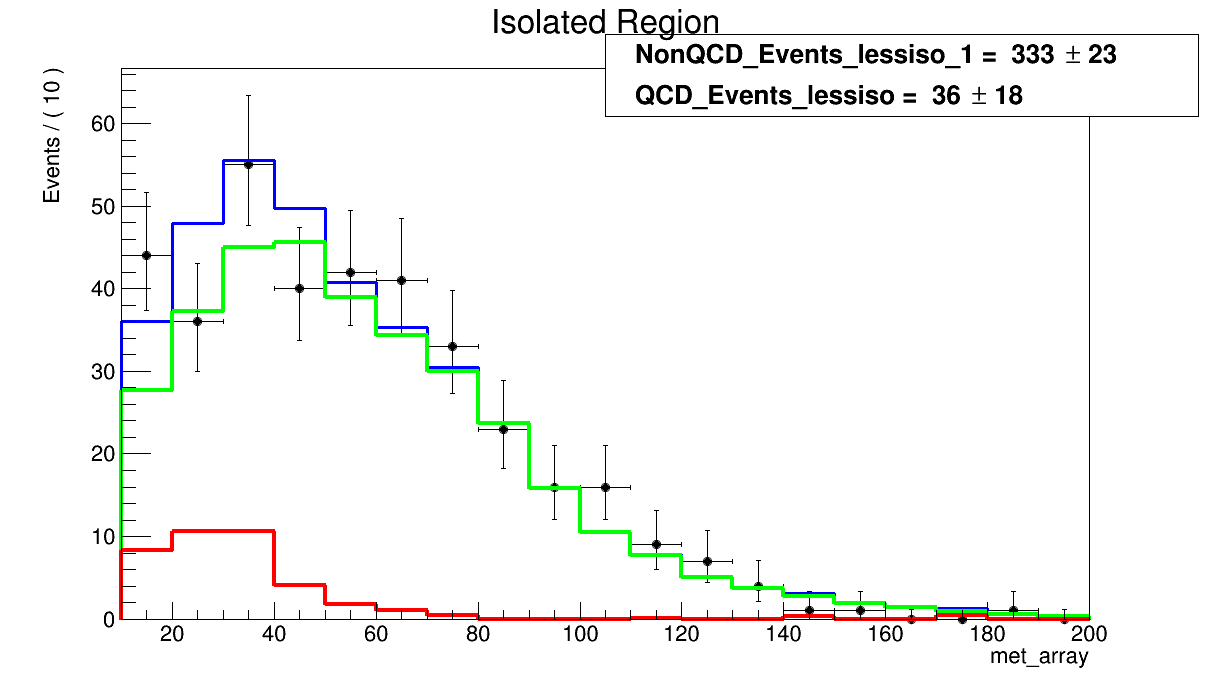
\includegraphics[scale=0.2]{figures/2J1T/MET_fit_2j1t_lessiso_SR}

\begin{centering}
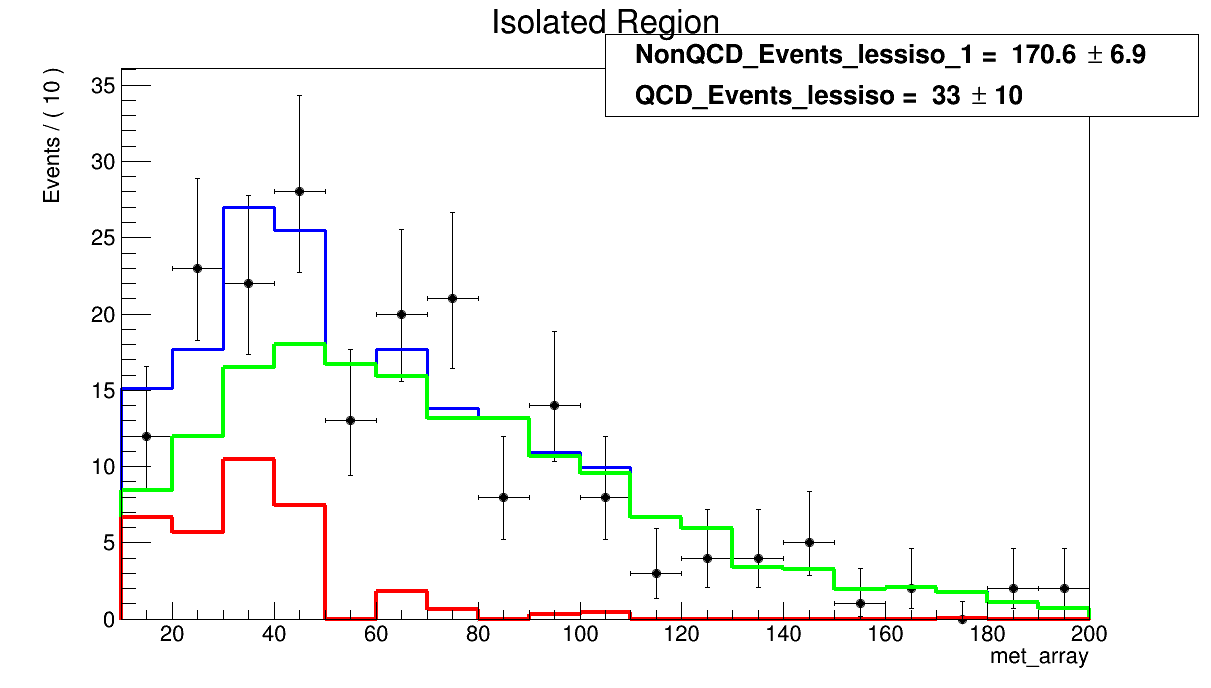
\includegraphics[scale=0.2]{figures/2J1T/MET_fit_2j1t_lessiso_SB}
\par\end{centering}
}
\resizebox{ \textwidth}{!}{
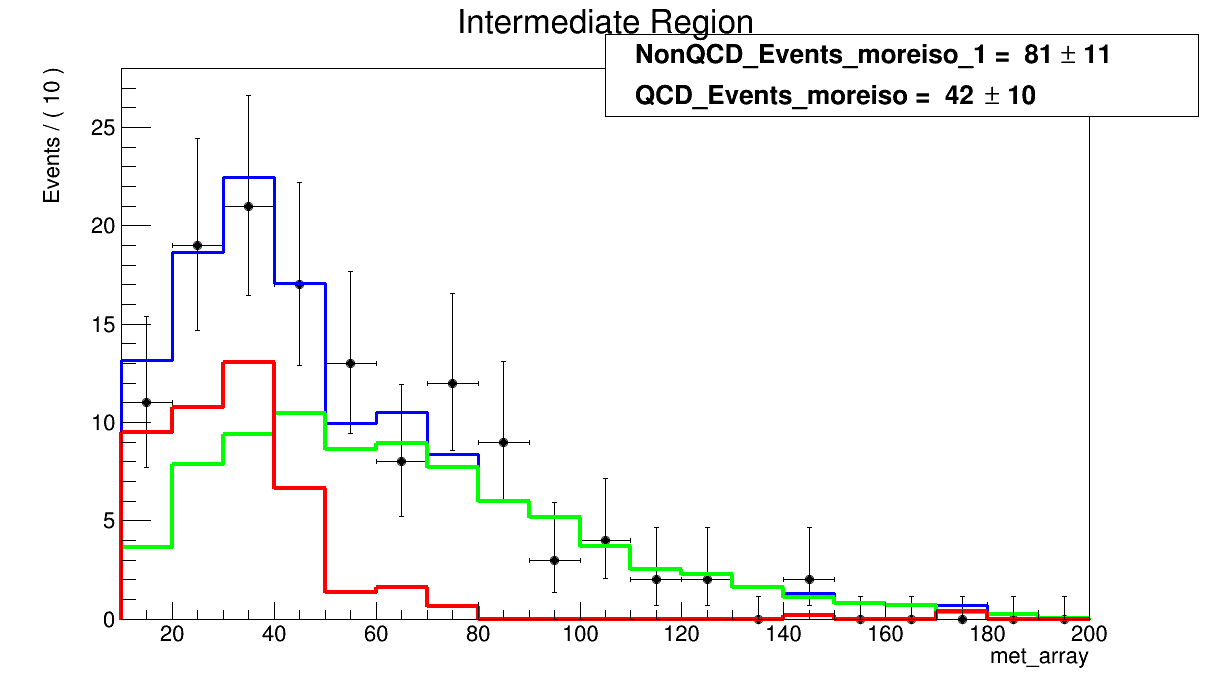
\includegraphics[scale=0.2]{figures/2J1T/MET_fit_2j1t_moreiso_inclusive_mTop_range}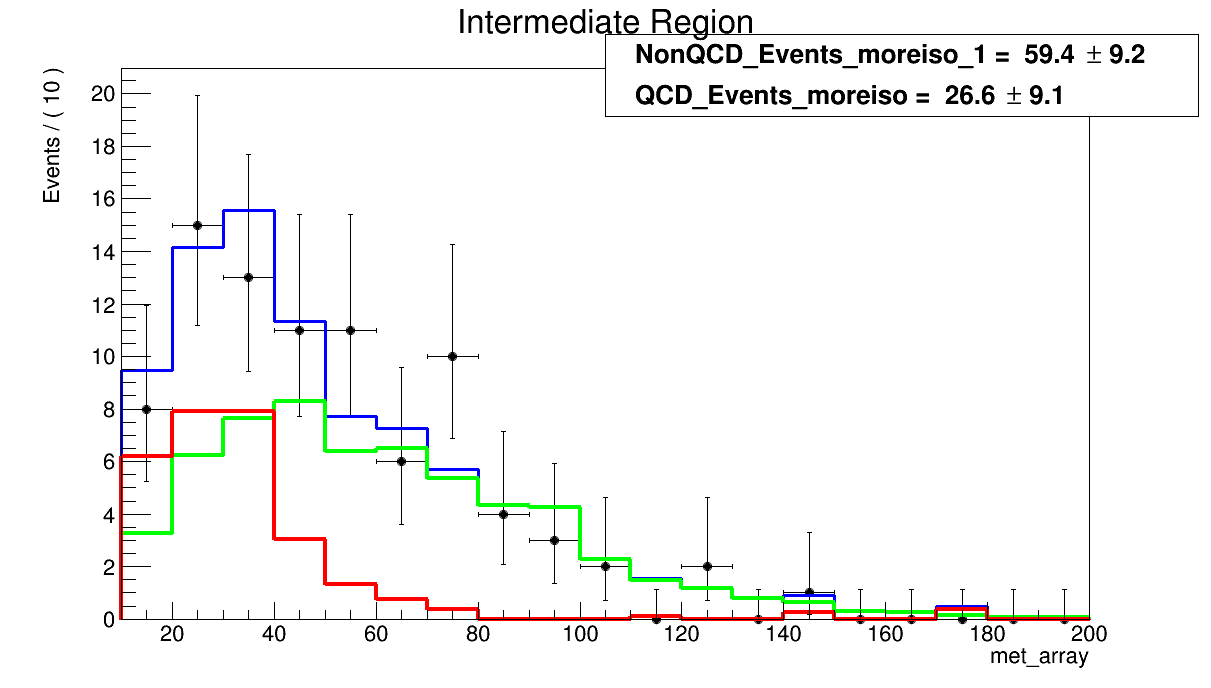
\includegraphics[scale=0.2]{figures/2J1T/MET_fit_2j1t_moreiso_SR}

\begin{centering}
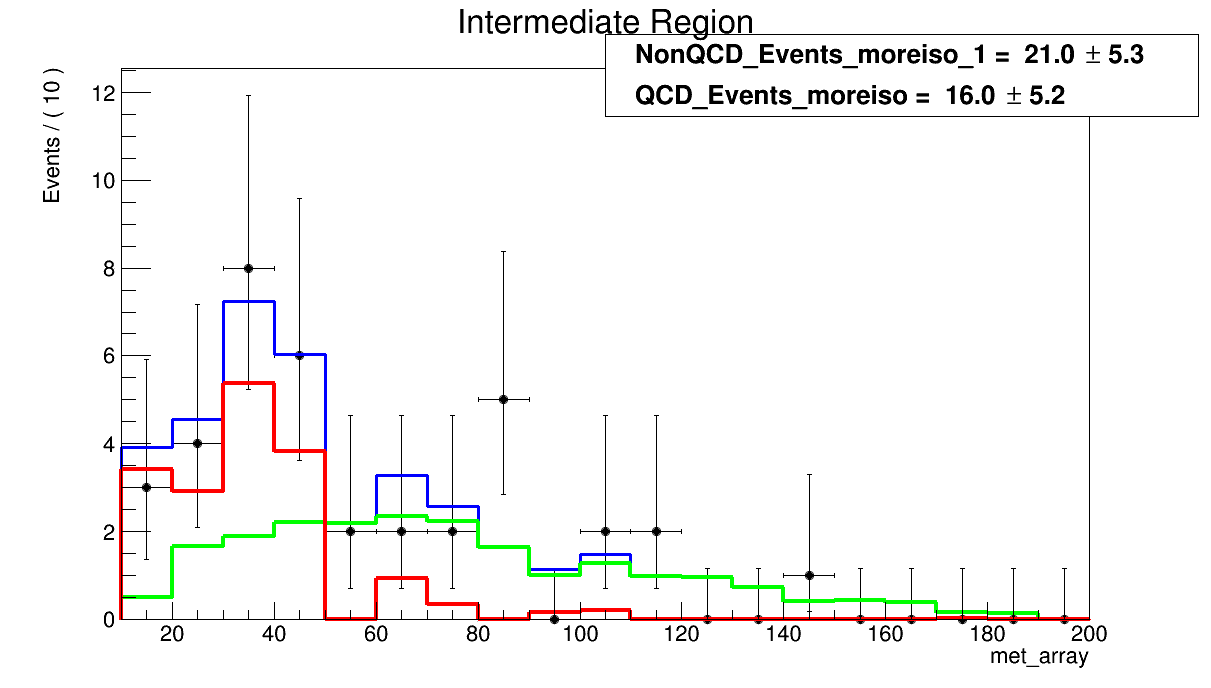
\includegraphics[scale=0.2]{figures/2J1T/MET_fit_2j1t_moreiso_SB}
\par\end{centering}
}
\caption{Fit to the $\met$ distribution in the \textquotedblleft{}2-jets
1-tag\textquotedblright{} sample inclusively (upper left), inside
(upper middle) and outside (upper right) the ${\rm m_{top}}$ window in
the signal region. Fit to the $\met$ distribution in the
\textquotedblleft{}2-jets 1-tag\textquotedblright{} sample inclusively
(bottom left), inside (bottom middle) and outside (bottom right) the ${\rm m_{top}}$
window in the intermediate-isolated region ($0.06 < \murelIso < 0.12$). }
\end{figure}


\clearpage

\subsection{Fit using the isolated region ($\PFrelIso < 0.12$)}

\begin{figure}[h!]
\resizebox{ \textwidth}{!}{
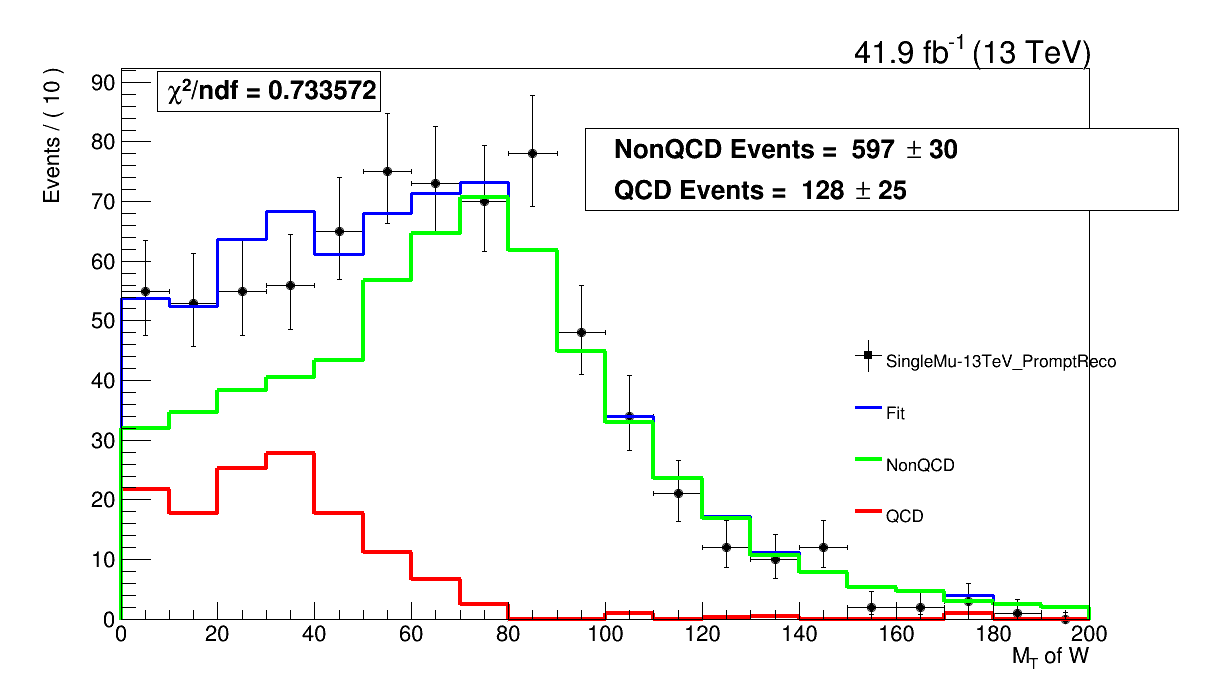
\includegraphics[scale=0.2]{figures/2J1T/MTW_fit_2j1t_iso_inclusive_mTop_range}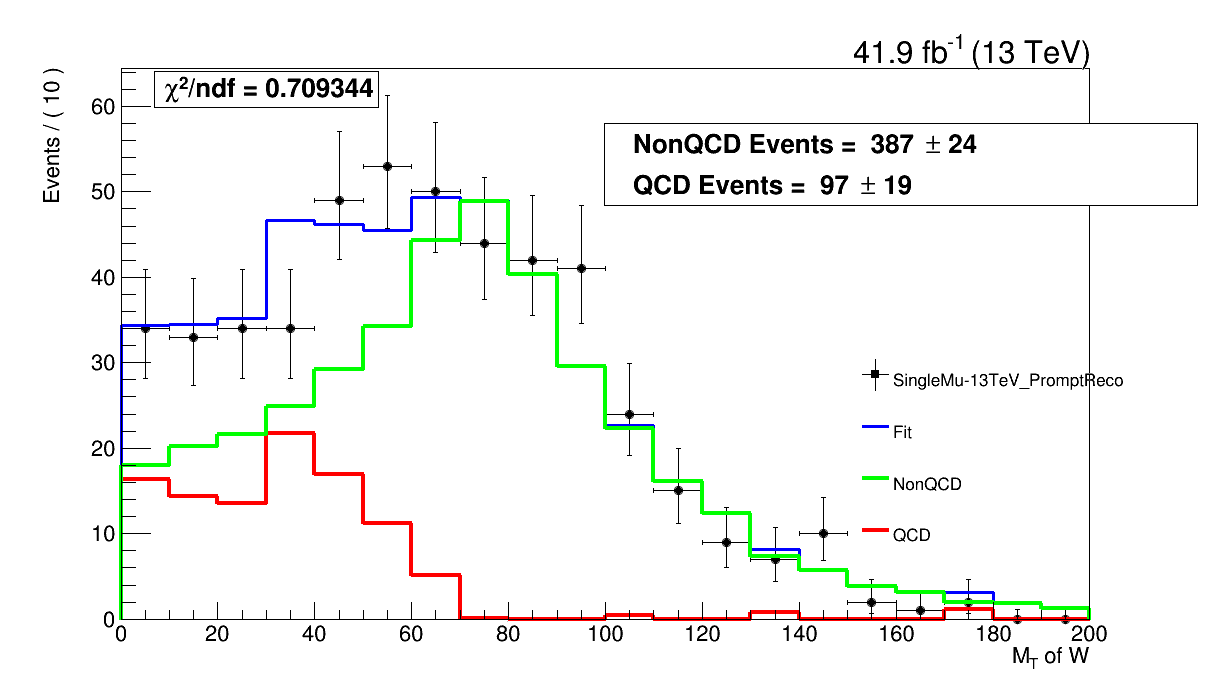
\includegraphics[scale=0.2]{figures/2J1T/MTW_fit_2j1t_iso_SR}

\begin{centering}
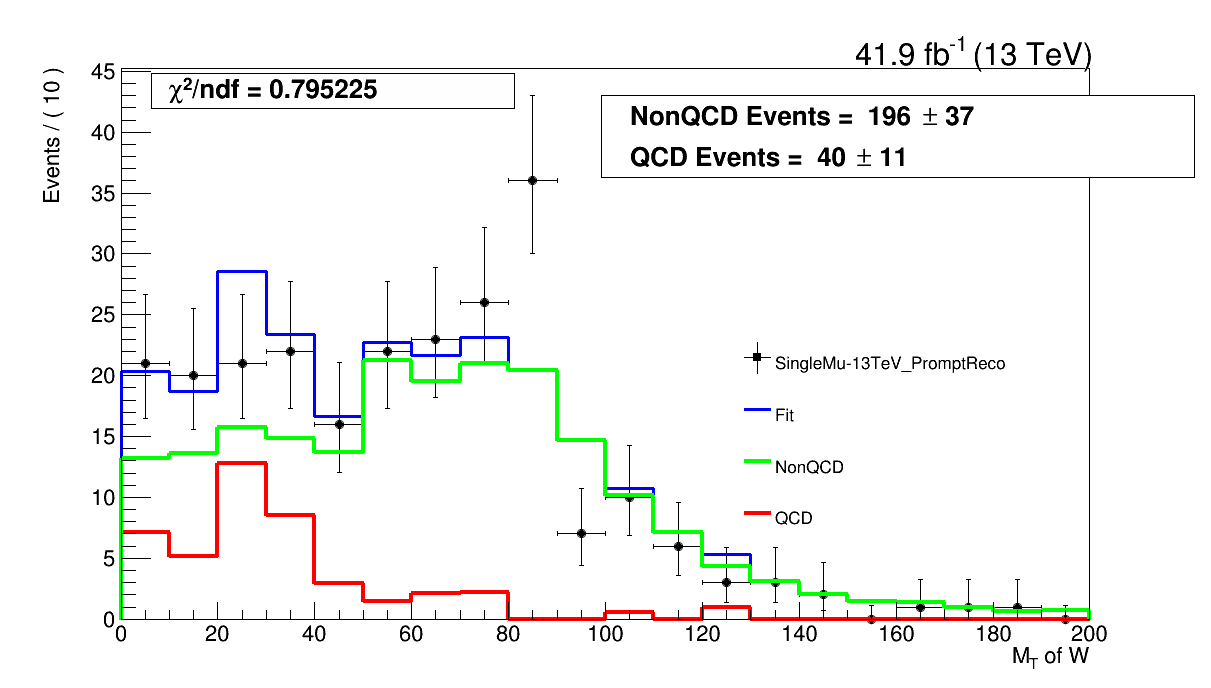
\includegraphics[scale=0.2]{figures/2J1T/MTW_fit_2j1t_iso_SB}
\par\end{centering}
}

\caption{Fit to the ${\rm m_{T}}$ distribution in the \textquotedblleft{}2-jets
1-tag\textquotedblright{} sample inclusively (upper left), inside
(upper middle) and outside (upper right) the ${\rm m_{top}}$ window in
the $\PFrelIso < 0.12$ isolated region.}
\end{figure}

\clearpage

%%%\subsection{Variation of anti-isolated region boundaries}

%%%To be added in the very next iteration.

\subsection{Fit with unbinned profile}

\begin{figure}[h!]
\centering{}

\resizebox{ \textwidth}{!}{
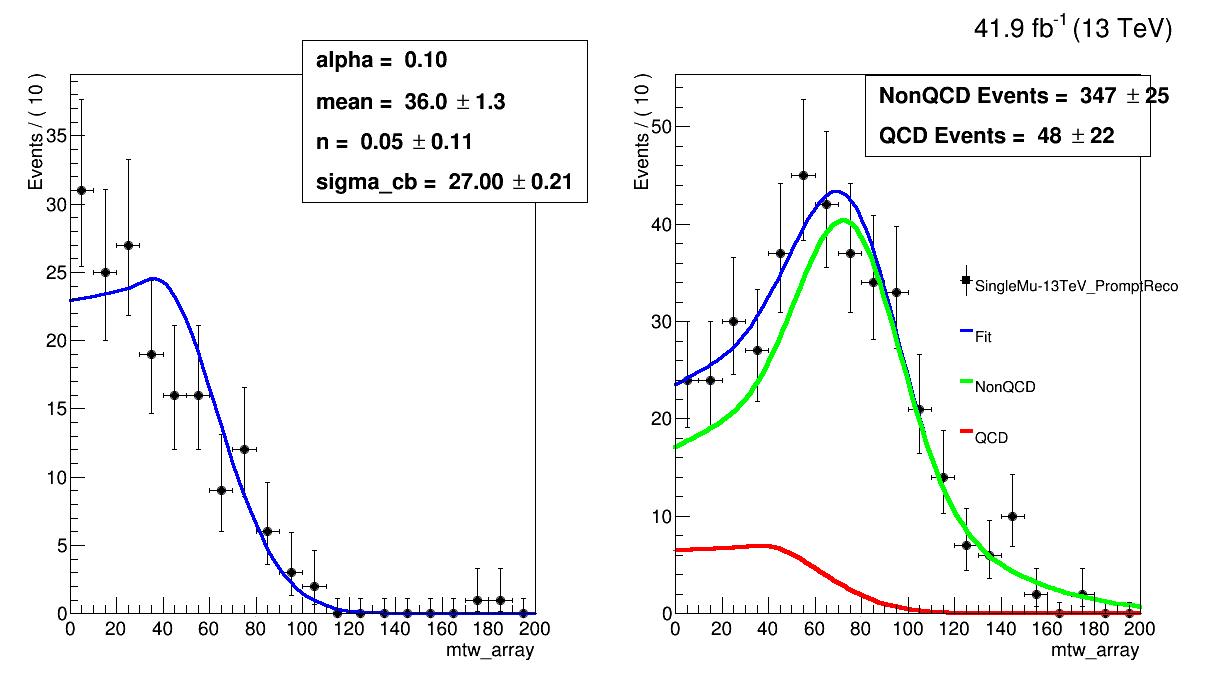
\includegraphics[scale=0.2]{figures/2J1T/MTW_unbinnedfit_2j1t_antiso_plus_lessiso_SR}
\begin{centering}
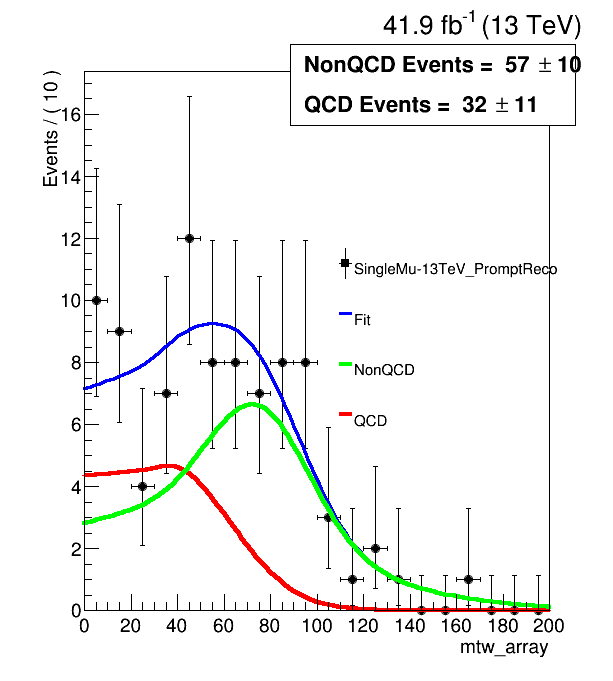
\includegraphics[scale=0.2]{figures/2J1T/MTW_unbinnedfit_2j1t_moreiso_SR}
\par\end{centering}
}


\resizebox{ \textwidth}{!}{
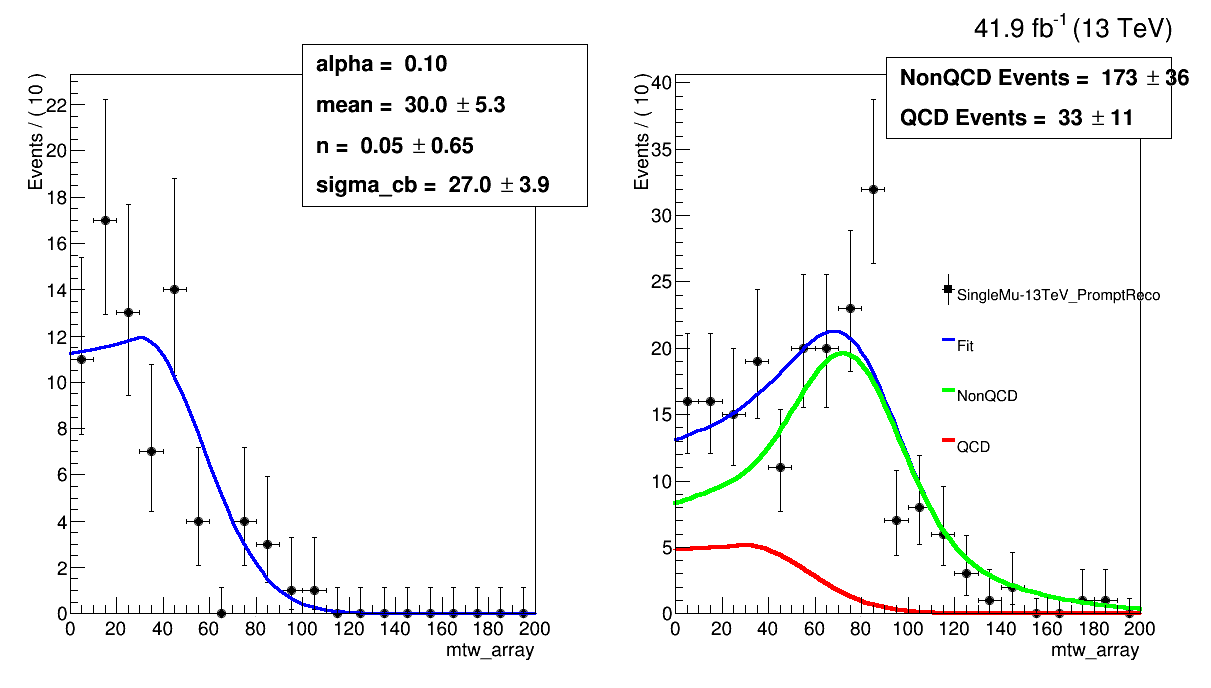
\includegraphics[scale=0.2]{figures/2J1T/MTW_unbinnedfit_2j1t_antiso_plus_lessiso_SB}
\begin{centering}
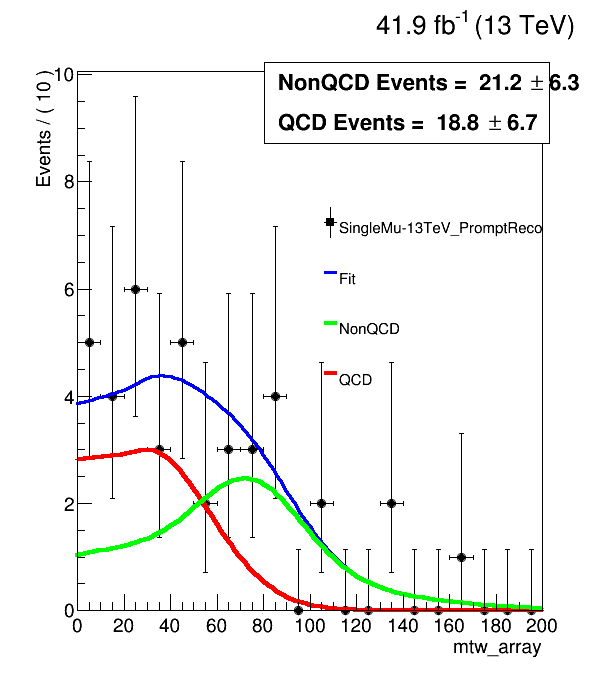
\includegraphics[scale=0.2]{figures/2J1T/MTW_unbinnedfit_2j1t_moreiso_SB}
\par\end{centering}
}

\resizebox{ \textwidth}{!}{
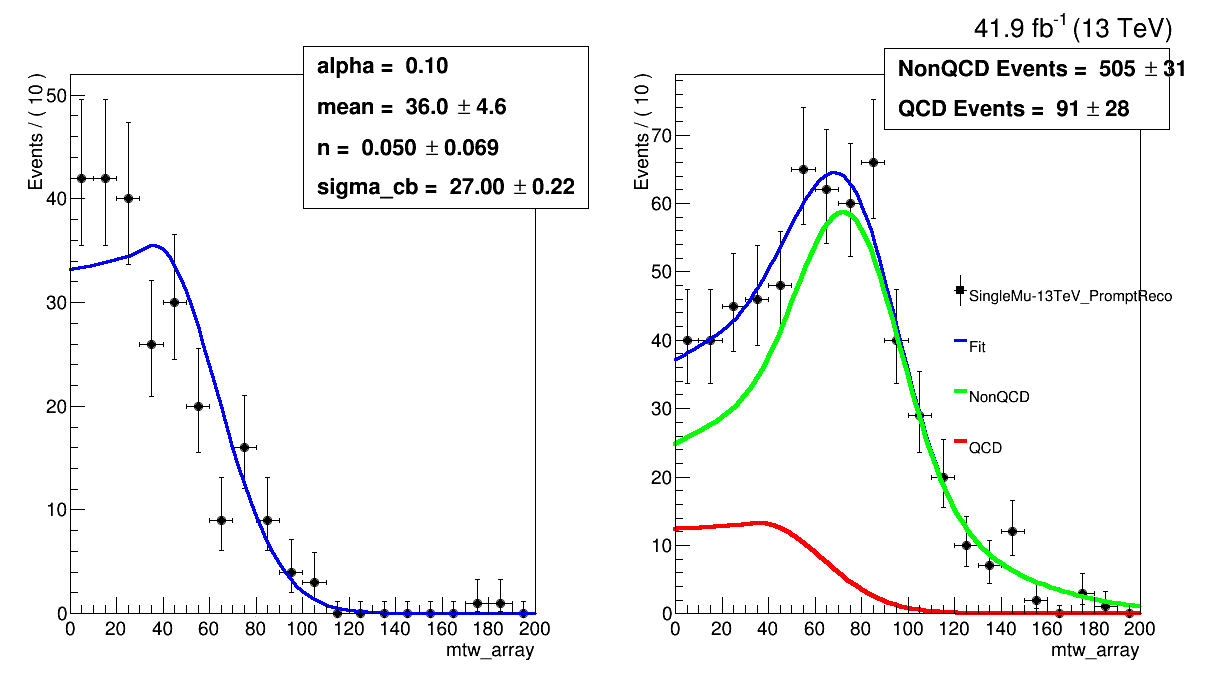
\includegraphics[scale=0.2]{figures/2J1T/MTW_unbinnedfit_2j1t_antiso_plus_lessiso_inclusive_mTop_range}
\begin{centering}
\includegraphics[scale=0.2]{figures/2J1T/MTW_unbinnedfit_2j1t_moreiso_inclusive_mTop_range}
\par\end{centering}
}


\caption{Unbinned fit to the ${\rm m_{T}}$ distribution the \textquotedblleft{}2-jets
1-tag\textquotedblright{} sample in the isolated (middle) and intermediate-isolated (right) region ($0.06 < \murelIso < 0.12$).
A Crystal Ball function has been selected to extract the QCD template
from the data in the anti-isolated region ($\murelIso > 0.12$) for both cases (left). An asymmetric
Gaussian has been selected to describe the non QCD template (Fig. ~\ref{fig:nonQCD_template_Unbinned}). From top to bottom: the SR ($130<\
\topMass<225\,$\GeV), the SB region and without applying any cut on $\topMass$.}
\end{figure}


\begin{figure}[h!]
\centering{}\includegraphics[scale=0.2]{figures/2J1T/MTW_unbinnedfit_variousmodels_2j1t_lessiso_inclusive_mTop_range_ttbar}\includegraphics[scale=0.2]{figures/2J1T/MTW_unbinnedfit_smoothkernel_2j1t_lessiso_inclusive_mTop_range_ttbar}\caption{\label{fig:nonQCD_template_Unbinned}Fit to the ${\rm m_{T}}$ distribution
of the \textquotedblleft{}2-jets 1-tag\textquotedblright{} (MC) sample
inclusively in the signal region. (left) The blue curve accounts
for an asymmetric Gaussian parameterization and has been fitted only
to the dominant ttbar MC background sample; this is the parameterization
that has been used in Table~\ref{tab:QCDEstimation2J1T}. The magenta curve corresponds to an
asymmetric Gaussian parameterization and has been fitted simultaneousnessly
to all MC background samples. The rest are estimations based on kernel
PDFs that promote precision (right) non QCD template estimation based
on kernel PDF that promotes smoothness.}
\end{figure}

\begin{table}[h!]

\caption{\scriptsize{isolated region ($\PFrelIso < 0.06$): Cross-check for systematic deviation on QCD yield for inclusive $\rm{m_{top}}$, SR and SB regions using unbinned profile; nominal values (on the left) are binned fit results having \bf{not} subtracted nonQCD}} \label{tab:Systematic_cross_check_QCD_yield_LessIso_NononQCDsubtraction} \centering %


\begin{tabular}{llccc} \hline\hline
	&	 & 	&\\ %
\multicolumn{2}{c}{Systematic \textit{Cross-Check}} & inclusive $\rm{m_{top}}$ & SR ($130<\rm{m_{top}}<225$ ) & SB \\
	&	 & 	&\\\hline %

\scriptsize{$|$nominal-variation($\pm$)$|$}   \\\hline

\scriptsize{Unbinned Profile} & \scriptsize{} & \scriptsize{$|$22(8)-27(8)$|$} & \scriptsize{$|$21(7)-14(6.6)$|$} & \scriptsize{$|$3(3.5)-8.16(2.7)$|$} \\\hline

\end{tabular} 
\end{table} 


\newline
\vspace*{1.5 cm}
\newline

\begin{table}[h!]

\caption{\scriptsize{intermediate region ($0.06 < \PFrelIso < 0.12$): Cross-check for systematic deviations on QCD yield for inclusive $\rm{m_{top}}$, SR and SB regions using unbinned profile; nominal values (on the left) are binned fit results having \bf{not} subtracted nonQCD }} \label{tab:Systematic_cross_check_QCD_yield_MoreIso_NononQCDsubtraction} \centering %

\begin{tabular}{llccc} \hline\hline
		&	 & 	&\\ %
	\multicolumn{2}{c}{Systematic \textit{Cross-Check}} & inclusive $\rm{m_{top}}$ & SR ($130<\rm{m_{top}}<225$ ) & SB \\
		&	 & 	&\\\hline %
	
	\scriptsize{$|$nominal-variation($\pm$)$|$}   \\\hline
	
	\scriptsize{Unbinned Profile} & \scriptsize{} & \scriptsize{$|$15(4)-16(3.9)$|$} & \scriptsize{$|$12(3)-9.5(3.3)$|$} & \scriptsize{$|$4(1.6)-4.65(1.65)$|$} \\\hline

\end{tabular} 
\end{table} 


\end{document}
